%%%%%%%%%%%%%%%%%%%%%%%%
% Sample use of the infthesis class to prepare an MSc thesis.
% This can be used as a template to produce your own thesis.
% Date: June 2019
%
%
% The first line specifies style options for taught MSc.
% You should add a final option specifying your degree.
% *Do not* change or add any other options.
%
% So, pick one of the following:
% \documentclass[msc,deptreport,adi]{infthesis}     % Adv Design Inf
% \documentclass[msc,deptreport,ai]{infthesis}      % AI
% \documentclass[msc,deptreport,cogsci]{infthesis}  % Cognitive Sci
% \documentclass[msc,deptreport,cs]{infthesis}      % Computer Sci
% \documentclass[msc,deptreport,cyber]{infthesis}   % Cyber Sec
% \documentclass[msc,deptreport,datasci]{infthesis} % Data Sci
% \documentclass[msc,deptreport,di]{infthesis}      % Design Inf
% \documentclass[msc,deptreport,inf]{infthesis}     % Informatics
%%%%%%%%%%%%%%%%%%%%%%%%

\documentclass[msc,deptreport.inf]{infthesis} % Do not change except to add your degree (see above).

% maths
\usepackage{amsmath}
\usepackage{amsfonts}
\usepackage{amssymb}
\newcommand{\matr}[1]{\mathbf{#1}}
\newcommand{\bgreek}[1]{\boldsymbol{#1}}
\newcommand{\R}{\mathbb R}
\newcommand{\E}{\mathbb E}
\newcommand{\V}{\mathbb V}
\newcommand{\N}{\mathbb N}
\newcommand{\diag}{\mathop{\mathrm{diag}}}

% algorithms
\usepackage{algorithm, algpseudocode}
\renewcommand{\algorithmicrequire}{\textbf{Input:}}
\renewcommand{\algorithmicensure}{\textbf{Output:}}

% graphics
\usepackage{graphicx}
\usepackage{subfig}


\begin{document}
\begin{preliminary}

\title{Extending the Bayesian Deep Learning Method MultiSWAG}

\author{Scott Brownlie}

\abstract{
  This skeleton demonstrates how to use the \texttt{infthesis} style
  for MSc dissertations in Artificial Intelligence, Cognitive Science,
  Computer Science, Data Science, and Informatics. It also emphasises
  the page limit, and that you must not deviate from the required
  style.  The file \texttt{skeleton.tex} generates this document and
  can be used as a starting point for your thesis. The abstract should
  summarise your report and fit in the space on the first page.
}

\maketitle

\section*{Acknowledgements}
Any acknowledgements go here.

\tableofcontents
\end{preliminary}


\chapter{Introduction}

The preliminary material of your report should contain:
\begin{itemize}
\item
The title page.
\item
An abstract page.
\item
Optionally an acknowledgements page.
\item
The table of contents.
\end{itemize}

As in this example \texttt{skeleton.tex}, the above material should be
included between:
\begin{verbatim}
\begin{preliminary}
    ...
\end{preliminary}
\end{verbatim}
This style file uses roman numeral page numbers for the preliminary material.

The main content of the dissertation, starting with the first chapter,
starts with page~1. \emph{\textbf{The main content must not go beyond page~40.}}

The report then contains a bibliography and any appendices, which may go beyond
page~40. The appendices are only for any supporting material that's important to
go on record. However, you cannot assume markers of dissertations will read them.

You may not change the dissertation format (e.g., reduce the font
size, change the margins, or reduce the line spacing from the default
1.5 spacing). Over length or incorrectly-formatted dissertations will
not be accepted and you would have to modify your dissertation and
resubmit.  You cannot assume we will check your submission before the
final deadline and if it requires resubmission after the deadline to
conform to the page and style requirements you will be subject to the
usual late penalties based on your final submission time.

%\section{Using Sections}
%
%Divide your chapters into sub-parts as appropriate.
%
%\section{Citations}
%
%Citations (such as \cite{P1} or \cite{P2}) can be generated using
%\texttt{BibTeX}. For more advanced usage, the \texttt{natbib} package is
%recommended. You could also consider the newer \texttt{biblatex} system.
%
%These examples use a numerical citation style. You may also use
%(Author, Date) format if you prefer.
%
%\chapter{Your next chapter}
%
%A dissertation usually contains several chapters.


\chapter{Background}\label{ch:background}

\section{Factor Analysis}\label{sec:fa}

Factor analysis (FA) is a latent variable model which generates observations $\theta \in \R^D$ as follows. First, a latent vector $\matr{h} \in \R^K$, for some $K < D$, is sampled from $p(\matr{h}) = \mathcal{N}(\matr{0}, \matr{I})$. Next, $\matr{h}$ is transformed onto a $K$-dimensional linear subspace of $\R^D$ by left-multiplying it by a \emph{factor loading} matrix $\matr{F} \in \R^{D \times K}$. The origin of this subspace is then shifted by adding a bias term $\matr{c} \in \R^D$. Finally, the data is perturbed by adding some zero mean Gaussian noise $\epsilon \in \R^D$ sampled from $\mathcal{N}(\matr{0}, \Psi)$, where $\Psi$ is a $D\times D$ diagonal matrix \cite{barber2007}. Putting all this together, an observation $\theta \in \R^D$ is generated according to 
\begin{equation}\label{eqn:fa_model}
	\theta = \matr{Fh} + \matr{c} + \epsilon.
\end{equation}
In the context of this thesis, an observation $\theta$ is the parameter vector of a neural network. 

It follows that, given $\matr{h}$, the observations $\theta$ are Gaussian distributed with mean $\matr{Fh} + \matr{c}$ and covariance $\Psi$ \cite{barber2007}. Formally,
\begin{equation}\label{eqn:fa_cond_dist}
	p(\theta | \matr{h}) 
	= \mathcal{N}\Big( \matr{Fh} + \matr{c}, \Psi \Big)
	= \frac{1}{\sqrt{(2\pi)^D |\Psi|}} 
	\exp \Big(-\frac{1}{2} (\theta - \matr{Fh} - \matr{c})^\intercal \Psi^{-1} (\theta - \matr{Fh} - \matr{c})\Big),
\end{equation}
where $|\Psi|$ is the \emph{determinant} of $\Psi$. From \cite{barber2007}, integrating $p(\theta | \matr{h})$ over $\matr{h}$ gives the marginal distribution
\begin{equation}\label{eqn:fa_marginal_dist}
	p(\theta) = \mathcal{N}\big(\matr{c}, \matr{FF}^{\intercal} + \Psi\big).
\end{equation}
The parameters of the model are $\matr{c}, \matr{F}$ and $\Psi$. The value of $\matr{c}$ which maximises the likelihood of the observed data is the empirical mean of the observations \cite{barber2007}, which in this case is $\theta_{\text{SWA}}$. 
%By substituting $\matr{c} = \theta_{\text{SWA}}$ into $p(\theta)$, the distribution in (\ref{eqn:fa_dist}) is obtained. 
Having set the bias term, an expectation-maximisation (EM) or singular value decomposition (SVD) algorithm can find the maximum likelihood estimates of $\matr{F}$ and $\Psi$ \cite{barber2007}. However, both methods require storing all the observations in memory, making them impractical for high-dimensional data, such as the parameter vectors of deep neural networks. Two alternative online algorithms are presented in Chapter \ref{ch:online_fa}.

\section{Bayesian Linear Regression}\label{sec:bayesian_lr}

A linear regression model is a mapping from vector inputs $\matr{x} \in \R^D$ to scalar outputs $y \in \R$ via an affine transformation. Given a set of observed input-output pairs, $\mathcal{D} = \{(\matr{x}_n, y_n)\}_{n=1}^{N}$, it is assumed that each output is generated according to 
\begin{equation}\label{eqn:linear_regression}
	y_n = \theta^\intercal \matr{x}_n + \epsilon
\end{equation}
for some unknown $\theta \in \R^D$. The underlying signal, $\theta^\intercal \matr{x}_n$, is corrupted by additive noise, 
\begin{equation}
	\epsilon \sim \mathcal{N}(0, \sigma^2), 
\end{equation}
for some $\sigma > 0$ \cite{barber2007}. The model is often written with an explicit bias term, but this can be absorbed into $\theta$ by adding a constant of one to the input, leading to the expression in Equation (\ref{eqn:linear_regression}).

\subsection{Computing the Posterior}

Due to the additive noise, each $y_n$ is a random variable, conditioned on $\matr{x}_n$ and $\theta$. Since $\epsilon$ is Gaussian distributed, the conditional pdf of $y_n$ is 
\begin{equation}\label{eqn:linear_regression_pdf}
	p(y_n | \theta, \matr{x}_n) 
	= \mathcal{N}\big(\theta^\intercal \matr{x}_n, \sigma^2\big)
	= \frac{1}{\sqrt{2\pi \sigma^2}} \exp\Big(-\frac{1}{2\sigma^2} \big(y_n - \theta^\intercal \matr{x}_n \big)^2\Big).
\end{equation}
Assuming that the observations in $\mathcal{D}$ are independent and identically distributed (iid), the log-likelihood of $\theta$ having generated the data is 
\begin{align}\label{eqn:linear_regression_log_likelihood}
\begin{split}
	\log p(\mathcal{D} | \theta) 
	& = \sum_{n=1}^N \big[ \log p(y_n | \theta, \matr{x}_n)  + \log p(\matr{x}_n) \big] \\
	& = \sum_{n=1}^N \Big[ -\frac{1}{2} \log 2\pi \sigma^2 - \frac{1}{2\sigma^2} \big(y_n - \theta^\intercal \matr{x}_n \big)^2 \Big]
	+ \sum_{n=1}^N \log p(\matr{x}_n) \\
	& = - \frac{1}{2 \sigma^2} \sum_{n=1}^N \big(y_n - \theta^\intercal \matr{x}_n \big)^2 
	- \frac{N}{2} \log \sigma^2
	- \frac{N}{2} \log 2\pi
	+ \sum_{n=1}^N \log p(\matr{x}_n) \\
	& = - \frac{\beta}{2} \sum_{n=1}^N \big(y_n - \theta^\intercal \matr{x}_n \big)^2 
	+ \frac{N}{2} \log \beta
	+ \text{constant},
\end{split}
\end{align}
where $\beta = \frac{1}{\sigma^2}$ \cite{barber2007}. In Bayesian linear regression, a prior distribution for $\theta$ is also specified. A common choice  is 
\begin{equation}\label{eqn:linear_regression_prior}
	p(\theta) 
	= \mathcal{N}\big(\matr{0}, \alpha^{-1} \matr{I} \big)
	= \Big(\frac{\alpha}{2\pi}\Big)^{\frac{D}{2}} \exp\Big(-\frac{\alpha}{2} \theta^\intercal \theta \Big)
\end{equation}
for some $\alpha > 0$, which is a hyperparameter known as the \emph{precision} \cite{barber2007}. Applying the logarithm, 
\begin{align}\label{eqn:linear_regression_log_prior}
\begin{split}
	\log p(\theta) 
	& = \frac{D}{2} \log \frac{\alpha}{2\pi} - \frac{\alpha}{2} \theta^\intercal \theta \\
	& = -\frac{\alpha}{2} \theta^\intercal \theta + \frac{D}{2} \log \alpha + \text{constant}.
\end{split}
\end{align}
Now, using Bayes' rule and Equation (\ref{eqn:linear_regression_log_likelihood}) and Equation (\ref{eqn:linear_regression_log_prior}), it follows that the log-posterior distribution of $\theta$ for fixed $\alpha$ and $\beta$ is 
\begin{align}\label{eqn:linear_regression_log_posterior}
\begin{split}
	\log p(\theta | \mathcal{D}) 
	& = \log \frac{p(\mathcal{D} | \theta) p(\theta)}{p(\mathcal{D})} \\
	& = \log p(\mathcal{D} | \theta) + \log p(\theta) - \log p(\mathcal{D}) \\
	& = -\frac{\beta}{2} \sum_{n=1}^N \big(y_n - \theta^\intercal \matr{x}_n \big)^2 
	-\frac{\alpha}{2} \theta^\intercal \theta 
	+ \text{constant} \\
	& = -\frac{\beta}{2} \sum_{n=1}^N\big( y_n^2 - 2 y_n \theta^\intercal \matr{x}_n + (\theta^\intercal \matr{x}_n)^2 \big)
	-\frac{\alpha}{2} \theta^\intercal \theta
	+ \text{constant} \\
	& = -\frac{\beta}{2} \sum_{n=1}^N y_n^2
	+ \beta \sum_{n=1}^N y_n \theta^\intercal \matr{x}_n
	-\frac{\beta}{2} \sum_{n=1}^N \theta^\intercal \matr{x}_n \matr{x}_n^\intercal \theta
	-\frac{\alpha}{2} \theta^\intercal \theta
	+ \text{constant} \\
	& = \Big(\beta \sum_{n=1}^N y_n \matr{x}_n \Big)^\intercal \theta 
	-\frac{1}{2} \theta^\intercal \Big( \alpha \matr{I} + \beta \sum_{n=1}^N \matr{x}_n \matr{x}_n^\intercal \Big) \theta 
	+ \text{constant} \\
	& = \matr{b}^\intercal \theta 
	- \frac{1}{2} \theta^\intercal \matr{A} \theta 
	+ \text{constant},
\end{split}
\end{align}
where 
\begin{equation}\label{eqn:linear_model_A_and_b}
	\matr{A} = \alpha \matr{I} + \beta \sum_{n=1}^N \matr{x}_n \matr{x}_n^\intercal
	\quad \text{and} \quad 
	\matr{b} = \beta \sum_{n=1}^N y_n \matr{x}_n.
\end{equation}
Now, using a result from \cite{barber2007} to complete the square of Equation (\ref{eqn:linear_regression_log_posterior}),
\begin{align}
\begin{split}
	\log p(\theta | \mathcal{D}) 
	& = -\frac{1}{2} \big(\theta - \matr{A}^{-1} \matr{b} \big)^\intercal \matr{A} \big(\theta - \matr{A}^{-1} \matr{b} \big)
	+ \frac{1}{2} \matr{b}^\intercal \matr{A}^{-1} \matr{b}
	+ \text{constant} \\
	& = -\frac{1}{2} \big(\theta - \matr{A}^{-1} \matr{b} \big)^\intercal \matr{A} \big(\theta - \matr{A}^{-1} \matr{b} \big)
	+ \text{constant} \\
	& = -\frac{1}{2} \big(\theta - \matr{m} \big)^\intercal \matr{S}^{-1} \big(\theta - \matr{m} \big)
	+ \text{constant},
\end{split}
\end{align}
where
\begin{equation}\label{eqn:linear_regression_posterior_params}
	\matr{m} = \matr{A}^{-1} \matr{b}
	\quad \text{and} \quad 
	\matr{S} = \matr{A}^{-1}.
\end{equation}
Hence, the posterior distribution of $\theta$ is 
\begin{align}\label{eqn:linear_regression_posterior}
\begin{split}
	p(\theta | \mathcal{D}) = \mathcal{N}(\matr{m}, \matr{S}).
\end{split}
\end{align}


\section{Gaussian Processes}\label{sec:gps}

%Linear regression is limited to modelling linear relationships between the inputs and output. 
%
%Gaussian processes (GPs) \cite{rasmussen2006} are a flexible class of non-parametric models. 

As in Section \ref{sec:bayesian_lr}, let $\mathcal{D} = \{(\matr{x}_n, y_n)\}_{n=1}^{N}$ be a set of training examples, where each $\matr{x}_n \in \R^D$ and $y_n \in \R$. Considering only the training set for now, a function $f$ can be specified by its values $\{f_n =  f(\matr{x}_n)\}_{n=1}^{N}$. Letting $\matr{f} = (f_1, \dots, f_N)^\intercal$, the function $f$ can be seen to generate a sample from a multivariate distribution. If this distribution is constrained to be Gaussian, then it is completely specified by the pdf
\begin{equation}
	p(\matr{f}) = \mathcal{N}(\mu, \Sigma)
\end{equation}
with parameters $\mu \in \R^D$ and $\Sigma \in \R^{D \times D}$. This is an example of a Gaussian process (GP), which is defined as a collection of random variables such that any finite number of the variables are jointly Gaussian \cite{rasmussen2006}. The finite subset in this case is $\{\matr{x}_n\}_{n=1}^{N}$, but any other set of inputs $\matr{x} \in \R^D$ would similarly give rise to a multivariate Gaussian distribution. 

The distribution $p(\matr{f})$ can be used as a prior on the function values of the training inputs before observing the outputs $y_n$. In the absence of domain knowledge about which function values are possible, a sensible choice for the prior mean is $\mu = \matr{0} \in \R^D$. By definition, the covariance matrix $\Sigma$ must be positive semi-definite. If $\Sigma$ was diagonal, function values $f_i$ and $f_j$, $i, j \in \{1, \dots, N\}$, would be independent, irrespective of how close $\matr{x}_i$ is to $\matr{x}_j$. This would lead to extremely noisy functions. To encourage smoothness, it is preferable to define a covariance matrix which assigns greater dependance between function values of nearby inputs. One way to generate covariance matrices with this property is by using the \emph{squared exponential kernel} function \cite{rasmussen2006}. Formally,
 \begin{equation}
	\Sigma_{i, j} = k(\matr{x}_i, \matr{x}_j) = \exp \Big( -\frac{1}{2} |\matr{x}_i - \matr{x}_j|^2 \Big).
\end{equation}
Different \emph{kernel} functions $k(\cdot, \cdot)$ give rise to different covariance matrices, and hence, different priors on the function values. 

To simplify the notation in what follows, let $\matr{X} \in \R^{N\times D}$ be formed by stacking $\matr{x}_1^\intercal,\dots,\matr{x}_N^\intercal$ in the rows of a matrix. Then the zero mean prior can be written as 
\begin{equation}
	p(\matr{f}) = \mathcal{N}(\matr{0}, K(\matr{X}, \matr{X})),
\end{equation}
where $K(\matr{A}, \matr{B})$, for $\matr{A} \in \R^{N\times D}$ and $\matr{B} \in \R^{M\times D}$, is shorthand from \cite{rasmussen2006} for the $N \times M$ matrix with elements
\begin{equation}
	K(\matr{A}, \matr{B})_{i, j} = k(\matr{a}_i, \matr{b}_j),
\end{equation} 
where $\matr{a}_i$ and $\matr{b}_j$ are the $i$-th and $j$-th rows of $\matr{A}$ and $\matr{B}$, respectively.


\subsection{Making Predictions with Gaussian Processes}

Suppose that the $y_n$ are noisy observations of the true function values at the training points. That is, $y_n = f_n + \epsilon$, where $\epsilon$ is iid zero mean Gaussian noise with variance $\sigma_y^2$. Letting $\matr{y} = (y_1, \dots, y_N)^\intercal$, the prior on $\matr{y}$ is 
\begin{equation}
	p(\matr{y}) = \mathcal{N}(\matr{0}, K(\matr{X}, \matr{X}) + \sigma_y^2 \matr{I}).
\end{equation}
Now suppose that $\matr{x}_{*} \in \R^D$ is a test point outside the training set. The prior on $f_{*} = f(\matr{x}_{*})$, the function value at the test point, is $p(f_{*} ) = \mathcal{N}(0, k(\matr{x}_{*}, \matr{x}_{*}))$. Hence, the joint distribution of the observed training outputs $\matr{y}$ and the test prediction $f_{*}$ is
\begin{equation}
	\begin{bmatrix}
		\matr{y} \\
		f_{*}
	\end{bmatrix}
	\sim \mathcal{N}\Bigg(
		\matr{0}, 
		\begin{bmatrix}
			K(\matr{X}, \matr{X}) + \sigma_y^2 \matr{I} & K(\matr{X}, \matr{x}_{*}) \\
			K(\matr{x}_{*}, \matr{X}) & k(\matr{x}_{*}, \matr{x}_{*})
		\end{bmatrix}
	\Bigg).
\end{equation}
Using a standard property of joint Gaussian distributions from \cite{barber2007}, the conditional distribution of $f_{*}$ given $\matr{y}$ is $p(f_{*} | \matr{y}) = \mathcal{N}(m, s^2)$, where
\begin{equation}
	m = K(\matr{x}_{*}, \matr{X}) \big[K(\matr{X}, \matr{X}) + \sigma_y^2 \matr{I}\big]^{-1} \matr{y}
\end{equation}
and
\begin{equation}
	s^2 = k(\matr{x}_{*}, \matr{x}_{*}) 
	- K(\matr{x}_{*}, \matr{X}) \big[K(\matr{X}, \matr{X}) + \sigma_y^2 \matr{I}\big]^{-1} K(\matr{X}, \matr{x}_{*}).
\end{equation}
Writing
\begin{equation}
	\matr{A} = \big[K(\matr{X}, \matr{X}) + \sigma_y^2 \matr{I}\big]^{-1}
	\quad \text{and} \quad 
	\matr{k}_{*} = K(\matr{X}, \matr{x}_{*}),
\end{equation}
the conditional distribution can be simplified to 
\begin{equation}\label{eqn:gp_prediction}
	p(f_{*} | \matr{y}) = \mathcal{N}\big(
		\matr{k}_{*}^\intercal \matr{A} \matr{y},  
		k(\matr{x}_{*}, \matr{x}_{*}) - \matr{k}_{*}^\intercal \matr{A} \matr{k}_{*}
	\big).
\end{equation} 


\subsection{Neural Network Kernel Function}

Let $f(\matr{x}): \R^D \mapsto \R$ be a neural network with a single hidden layer. Neural network will be explained in more detail in Section \ref{sec:dnns}, but for now it is enough to know that the functional form of the single layer model is
\begin{equation}
	f(\matr{x}) = b + \sum_{h=1}^H v_h \cdot g(\matr{w}_h^\intercal \matr{x}),
\end{equation} 
where $H$ is the number of \emph{units} in the hidden layer, the $\matr{w}_h \in \R^D$ and $v_h, b \in \R$ are learnable parameters and $g(x):\R \mapsto \R$ is a non-linear \emph{activation} function \cite{goodfellow2016}. Here $\matr{x}$ has been augmented with a constant of one such that the bias term of each hidden unit is absorbed into the corresponding $\matr{w}_h$.

Let $\theta \in \R^{Dh + h + 1}$ denote all the learnable parameters of the neural network. For any two points $\matr{x}, \matr{x}' \in \R^D$, the covariance of their predictions is 
\begin{equation}\label{eqn:nn_cov}
	\E_{p(\theta)}\Big[\big(f(\matr{x}) - \E_{p(\theta)}[f(\matr{x})]\big) \big(f(\matr{x}') - \E_{p(\theta)}[f(\matr{x}')]\big)\Big].
\end{equation} 
Assuming that $b \sim \mathcal{N}(0, \sigma_b^2)$ and $v_h \sim \mathcal{N}(0, \sigma_v^2)$ are independent and that the $\matr{w}_h \sim p(\matr{w}) = \mathcal{N}(\matr{0}, \Sigma_{\matr{w}})$ are iid for each hidden unit, Equation (\ref{eqn:nn_cov}) can be written as 
\begin{equation}\label{eqn:simplified_nn_cov}
	\sigma_b^2 + H \sigma_v^2 \E_{p(\matr{w})} \big[ g(\matr{w}^\intercal \matr{x}) g(\matr{w}^\intercal \matr{x}') \big],
\end{equation} 
where $\matr{w}$ replaces $\matr{w}_h$ due to the iid assumption \cite{williams1997}. Moreover, as $H \rightarrow \infty$, the neural network will converge to a GP \cite{williams1997}. Of course, for this to be a valid GP the activation function $g$ must give rise to a positive definite kernel. One suitable activation is the \emph{error function}, 
\begin{equation}
	\text{erf}(z) = \frac{2}{\sqrt{\pi}} \int_0^z e^{-t^2} dt.
\end{equation}
Setting $g = \text{erf}$ and evaluating $\E_{p(\matr{w})} \big[ \text{erf}(\matr{w}^\intercal \matr{x}) \text{erf}(\matr{w}^\intercal \matr{x}') \big]$, it is shown in \cite{williams1997} that the kernel function of this neural network is
\begin{equation}\label{eqn:nn_kernel}
	k_{\text{NN}}(\matr{x}, \matr{x}') = \frac{2}{\pi} \sin^{-1} 
	\Bigg( \frac{2\matr{x}^\intercal \Sigma_{\matr{w}} \matr{x}'}{\sqrt{(1 + 2\matr{x}^\intercal \Sigma_{\matr{w}} \matr{x}) (1 + 2\matr{x}'^\intercal \Sigma_{\matr{w}} \matr{x}')}} \Bigg).
\end{equation}



\section{Deep Neural Networks}\label{sec:dnns}


\chapter{Related Work and Research Questions}\label{ch:previous_work}


\chapter{Online Factor Analysis}\label{ch:online_fa}


\section{Online Stochastic Gradient Ascent}\label{sec:gradient_fa}

In situations where learning latent variable models with the classic EM algorithm is slow, \cite{barber2007} suggests optimising the log-likelihood of the model parameters via gradient methods. Since FA is a latent variable model, this approach can be applied here. 

In this case, the log-likelihood of the parameters $\matr{F}$ and $\Psi$ given the observed data, $\theta_1,\dots,\theta_T$, is 
\begin{equation}
	L(\matr{F}, \Psi) = \frac{1}{T} \sum_{t=1}^T \log p(\theta_t | \matr{F}, \Psi).
\end{equation}
The partial derivatives of the log-likelihood with respect to $\matr{F}$ and $\Psi$ are therefore
\begin{equation}
	\nabla_{\matr{F}, \Psi} L(\matr{F}, \Psi) = \frac{1}{T} \sum_{t=1}^T \nabla_{\matr{F}, \Psi} \log p(\theta_t | \matr{F}, \Psi).
\end{equation}
Computing $\nabla_{\matr{F}, \Psi} L(\matr{F}, \Psi)$ in full would require a pass over all observations, $\theta_1, \dots, \theta_T$. However, a stochastic gradient algorithm can be used instead, as long as the expectation of the sample derivatives is proportional to $\nabla_{\matr{F}, \Psi} L(\matr{F}, \Psi)$. By using $\nabla_{\matr{F}, \Psi} \log p(\theta_t | \matr{F}, \Psi)$, $t=1,\dots,T$, as the sample derivatives, this condition clearly holds. Hence, as long as the partial derivatives $\nabla_{\matr{F}, \Psi} \log p(\theta_t | \matr{F}, \Psi)$ can be computed efficiently, they can be used in conjunction with SGD or any of its variants to optimise $\matr{F}$ and $\Psi$ online. 
%After each $\theta_t$ is sampled and used to perform a gradient step, it can immediately be discarded. 

By adapting an argument for general latent variable models in \cite{barber2007} to FA, the required sample derivatives can be written as
\begin{align}\label{eqn:grad_log_likelihood}
\begin{split}
	\nabla_{\matr{F}, \Psi} \log p(\theta_t | \matr{F}, \Psi) 
	& = \frac{1}{p(\theta_t | \matr{F}, \Psi)} \nabla_{\matr{F}, \Psi} p(\theta_t | \matr{F}, \Psi) \\
	& = \frac{1}{p(\theta_t | \matr{F}, \Psi)} \nabla_{\matr{F}, \Psi} \int_{\matr{h}_t} p(\theta_t, \matr{h}_t | \matr{F}, \Psi) \\
	& = \frac{1}{p(\theta_t | \matr{F}, \Psi)} \int_{\matr{h}_t} \nabla_{\matr{F}, \Psi} p(\theta_t, \matr{h}_t | \matr{F}, \Psi) \\
	& = \frac{1}{p(\theta_t | \matr{F}, \Psi)} \int_{\matr{h}_t} p(\theta_t, \matr{h}_t | \matr{F}, \Psi) \nabla_{\matr{F}, \Psi} \log p(\theta_t, \matr{h}_t | \matr{F}, \Psi) \\
	& = \int_{\matr{h}_t} \frac{p(\theta_t, \matr{h}_t | \matr{F}, \Psi)}{p(\theta_t | \matr{F}, \Psi)} \nabla_{\matr{F}, \Psi} \log p(\theta_t, \matr{h}_t | \matr{F}, \Psi) \\
	& = \int_{\matr{h}_t} p(\matr{h}_t | \theta_t, \matr{F}, \Psi) \nabla_{\matr{F}, \Psi} \log p(\theta_t, \matr{h}_t | \matr{F}, \Psi) \\
	& = \E_{p(\matr{h}_t | \theta_t, \matr{F}, \Psi)} \big[ \nabla_{\matr{F}, \Psi} \log p(\theta_t, \matr{h}_t | \matr{F}, \Psi) \big].
\end{split}
\end{align}
This is as far as the derivation in \cite{barber2007} goes. However, given the form of the FA model, it is possible to manipulate the sample derivatives further. In particular, using the fact that $\matr{h}_t \sim \mathcal{N}(\matr{0}, \matr{I})$ is independent from $\matr{F}$ and $\Psi$,
\begin{align}\label{eqn:grad_log_complete_likelihood}
\begin{split}
	\nabla_{\matr{F}, \Psi} \log p(\theta_t, \matr{h}_t | \matr{F}, \Psi)
	& = \nabla_{\matr{F}, \Psi} \log \big(p(\theta_t | \matr{h}_t, \matr{F}, \Psi)p(\matr{h}_t | \matr{F}, \Psi)\big) \\
	& = \nabla_{\matr{F}, \Psi} \log \big(p(\theta_t | \matr{h}_t, \matr{F}, \Psi)p(\matr{h}_t)\big) \\
	& = \nabla_{\matr{F}, \Psi} \big( \log p(\theta_t | \matr{h}_t, \matr{F}, \Psi) + \log p(\matr{h}_t)\big) \\
	& = \nabla_{\matr{F}, \Psi} \log p(\theta_t | \matr{h}_t, \matr{F}, \Psi).
\end{split}
\end{align}
Substituting Equation (\ref{eqn:grad_log_complete_likelihood}) into Equation (\ref{eqn:grad_log_likelihood}),
\begin{equation}\label{eqn:simplified_grad_log_likelihood}
	\nabla_{\matr{F}, \Psi} \log p(\theta_t | \matr{F}, \Psi)
	= \E_{p(\matr{h}_t | \theta_t, \matr{F}, \Psi)} \big[ \nabla_{\matr{F}, \Psi} \log p(\theta_t | \matr{h}_t, \matr{F}, \Psi) \big].
\end{equation}
Note that $p(\theta_t | \matr{h}_t, \matr{F}, \Psi)$ is just the Gaussian distribution in Equation (\ref{eqn:fa_cond_dist}), given $\matr{F}$ and $\Psi$. Hence, substituting $\matr{c} = \theta_{\text{SWA}}$ into Equation (\ref{eqn:fa_cond_dist}) and applying the logarithm,
\begin{align}\label{eqn:log_fa_cond_dist}
\begin{split}
	\log p(\theta_t | \matr{h}_t, \matr{F}, \Psi)
	& = -\frac{1}{2} (\theta_t - \matr{Fh}_t - \theta_{\text{SWA}})^\intercal \Psi^{-1} (\theta_t - \matr{Fh}_t - \theta_{\text{SWA}}) - \frac{1}{2} \log |\Psi| - \frac{D}{2} \log 2\pi \\
	& = -\frac{1}{2} (\matr{d}_t - \matr{Fh}_t)^\intercal \Psi^{-1} (\matr{d}_t - \matr{Fh}_t) - \frac{1}{2} \log |\Psi| - \frac{D}{2} \log 2\pi,
\end{split}
\end{align}
where $\matr{d}_t = \theta_t - \theta_{\text{SWA}}$. This is convenient, since Equation (\ref{eqn:log_fa_cond_dist}) can be differentiated with respect to both $\matr{F}$ and $\Psi$. Of course, this requires access to $\theta_{\text{SWA}}$, which is not available during training. As a compromise - and following the approach of the SWAG covariance approximation - $\theta_{\text{SWA}}$ can be replaced by the running average of the neural network's parameter vectors.

\subsection{Partial derivatives with respect to $\matr{F}$}

From \cite{petersen2012}, for any symmetric matrix $\matr{W}$,
\begin{equation}
	\nabla_{\matr{A}} (\matr{x} - \matr{As})^\intercal \matr{W} (\matr{x} - \matr{As}) = -2 \matr{W} (\matr{x} - \matr{As}) \matr{s}^\intercal.
\end{equation}
Hence, differentiating Equation (\ref{eqn:log_fa_cond_dist}) with respect to $\matr{F}$ gives
\begin{equation}
	\nabla_{\matr{F}} \log p(\theta_t | \matr{h}_t, \matr{F}, \Psi)
	= \Psi^{-1} (\matr{d}_t - \matr{Fh}_t) \matr{h}_t^\intercal.
\end{equation}
It then follows from Equation (\ref{eqn:simplified_grad_log_likelihood}) that $\nabla_{\matr{F}} \log p(\theta_t | \matr{F}, \Psi)$ is the expected value of $\Psi^{-1} (\matr{d}_t - \matr{Fh}_t) \matr{h}_t^\intercal$ over the distribution $p(\matr{h}_t | \theta_t, \matr{F}, \Psi)$. Letting $\E[\cdot]$ denote $\E_{p(\matr{h}_t | \theta_t, \matr{F}, \Psi)}[\cdot]$ to simplify the notation, 
\begin{align}\label{eqn:expected_derivatives_wrt_F}
\begin{split}
	\nabla_{\matr{F}} \log p(\theta_t | \matr{F}, \Psi) 
	& = \E \big[ \Psi^{-1} (\matr{d}_t - \matr{Fh}_t) \matr{h}_t^\intercal \big] \\
	& = \Psi^{-1} \big(\E \big[ \matr{d}_t \matr{h}_t^\intercal \big] 
	- \E \big[ \matr{Fh}_t \matr{h}_t^\intercal \big] \big) \\
	& = \Psi^{-1}\big( \matr{d}_t \E \big[ \matr{h}_t^\intercal \big] 
	- \matr{F}  \E \big[ \matr{h}_t \matr{h}_t^\intercal \big]\big).
\end{split}
\end{align} 
From the E-step of the EM algorithm for FA in \cite{barber2007}, $p(\matr{h}_t | \theta_t, \matr{F}, \Psi) \propto \mathcal{N}(\matr{m}_t, \Sigma)$, where
\begin{equation}\label{eqn:variational_params}
	\Sigma = (\matr{I} + \matr{F}^\intercal \Psi^{-1} \matr{F})^{-1}
	\quad \text{and} \quad \matr{m}_t = \Sigma \matr{F}^\intercal \Psi^{-1} \matr{d}_t.
\end{equation}
Hence, using identities from \cite{petersen2012}, 
\begin{equation}\label{eqn:expected_value_h_hh}
	\E \big[ \matr{h}_t^\intercal \big] = \matr{m}_t^\intercal \quad \text{and} \quad \E \big[ \matr{h}_t \matr{h}_t^\intercal \big] = \Sigma + \matr{m}_t \matr{m}_t^\intercal.
\end{equation}
Finally, substituting Equation (\ref{eqn:expected_value_h_hh}) into Equation (\ref{eqn:expected_derivatives_wrt_F}), 
\begin{align}\label{eqn:derivatives_wrt_F}
\begin{split}
	\nabla_{\matr{F}} \log p(\theta_t | \matr{F}, \Psi) 
	& = \Psi^{-1} \big(\matr{d}_t \matr{m}_t^\intercal - \matr{F}  (\Sigma + \matr{m}_t \matr{m}_t^\intercal)\big).
\end{split}
\end{align} 

\subsection{Partial derivatives with respect to $\Psi$}

In order to differentiate Equation (\ref{eqn:log_fa_cond_dist}) with respect to $\Psi$, it helps to use the fact that $\Psi$ is diagonal. First consider $\matr{X}^{-1} = \diag(\frac{1}{x_1}, \dots, \frac{1}{x_D})$ and $\matr{a} = (a_1, \dots, a_D)^\intercal$. Then 
\begin{equation}\label{eqn:aXa}
	\matr{a}^\intercal \matr{X}^{-1} \matr{a} = \sum_{d=1}^D \frac{a_d^2}{x_d},
\end{equation}
and so
\begin{equation}
	\frac{\partial}{\partial x_d} \matr{a}^\intercal \matr{X}^{-1} \matr{a} = \frac{-a_d^2}{x_d^2}
\end{equation}
for $d=1, \dots, D$. Since the partial derivatives of Equation (\ref{eqn:aXa}) with respect to the off-diagonal entries of $\matr{X}$ are zero, 
\begin{align}\label{eqn:derivatives_diag_qaud_form}
\begin{split}
	\nabla_\matr{X} (\matr{a}^\intercal \matr{X}^{-1} \matr{a}) 
	& = \diag\Big({\frac{-a_1^2}{x_1^2}, \dots, \frac{-a_D^2}{x_D^2}}\Big) \\
	& = -\diag\big(\diag(\matr{X}^{-2}) \odot \matr{a}^2\big),
\end{split}
\end{align}  
where $\odot$ denotes the element-wise matrix product (with broadcasting, if applicable) and the square of a vector is applied element-wise. Also, when applied to a $D$-length vector, $\diag(\cdot)$ represents the $D \times D$ diagonal matrix with the vector on its diagonal, and when applied to a $D \times D$ matrix, $\diag(\cdot)$ represents the $D$-length vector consisting of the diagonal entries of the matrix. Substituting $\matr{X} = \Psi$ and $\matr{a} = \matr{d}_t - \matr{Fh}_t$, into Equation (\ref{eqn:derivatives_diag_qaud_form}),
\begin{equation}\label{eqn:derivatives_wrt_Psi_1}
	\nabla_\Psi (\matr{d}_t - \matr{Fh}_t)^\intercal \Psi^{-1} (\matr{d}_t - \matr{Fh}_t) 
	= -\diag\big(\diag(\Psi^{-2}) \odot (\matr{d}_t - \matr{Fh}_t)^2\big).
\end{equation}
Also, using the identity $\nabla_\matr{X} \log |\matr{X}| = \matr{X}^{-\intercal}$ from \cite{petersen2012} and the fact that $\Psi^{-\intercal} = \Psi^{-1}$, 
\begin{equation}\label{eqn:derivatives_wrt_Psi_2}
	\nabla_\Psi \log |\Psi|
	= \Psi^{-1}.
\end{equation}
Hence, the partial derivatives of Equation (\ref{eqn:log_fa_cond_dist}) with respect to $\Psi$ are
\begin{equation}
	\nabla_{\Psi} \log p(\theta_t | \matr{h}_t, \matr{F}, \Psi)
	= \frac{1}{2} \diag\big(\diag(\Psi^{-2}) \odot (\matr{d}_t - \matr{Fh}_t)^2\big) - \frac{1}{2}\Psi^{-1}.
\end{equation}
Again, letting $\E[\cdot]$ denote $\E_{p(\matr{h}_t | \theta_t, \matr{F}, \Psi)}[\cdot]$, it follows from Equation (\ref{eqn:simplified_grad_log_likelihood}) that
\begin{align}\label{eqn:expected_gradient}
\begin{split}
	2 \cdot \nabla_{\Psi} \log p(\theta_t | \matr{F}, \Psi) 
	& = \E \big[ \diag\big(\diag(\Psi^{-2}) \odot (\matr{d}_t - \matr{Fh}_t)^2\big) - \Psi^{-1} \big] \\
	& = \diag\Big(\E \big[\diag(\Psi^{-2}) \odot (\matr{d}_t - \matr{Fh}_t)^2\big]\Big) - \E \big[ \Psi^{-1} \big] \\
	& = \diag\Big(\diag(\Psi^{-2}) \odot \E \big[(\matr{d}_t - \matr{Fh}_t)^2\big]\Big) - \Psi^{-1}.
\end{split}
\end{align} 
Now, expanding the expectation inside Equation (\ref{eqn:expected_gradient}) and substituting in the expressions from Equation (\ref{eqn:expected_value_h_hh}),
\begin{align}\label{eqn:expected_gradient_d_Fh}
\begin{split}
	\E \big[(\matr{d}_t - \matr{Fh}_t)^2\big] 
	& = \E \big[\matr{d}_t \odot \matr{d}_t \big] - 2\E \big[ \matr{d}_t \odot (\matr{Fh}_t) \big] + \E \big[ (\matr{Fh}_t) \odot (\matr{Fh}_t) \big] \\
	& = \matr{d}_t \odot \matr{d}_t - 2\matr{d}_t \odot \big(\matr{F} \E \big[ \matr{h}_t \big]\big) + \E \big[ \diag(\matr{F}\matr{h}_t \matr{h}_t^\intercal  \matr{F}^\intercal) \big] \\
	& = \matr{d}_t \odot \matr{d}_t - 2\matr{d}_t \odot (\matr{F} \matr{m}_t) + \diag\big(\E \big[ \matr{F}\matr{h}_t \matr{h}_t^\intercal  \matr{F}^\intercal \big]\big) \\
	& = \matr{d}_t \odot \matr{d}_t - 2\matr{d}_t \odot (\matr{F} \matr{m}_t) + \diag\big( \matr{F} \E \big[ \matr{h}_t \matr{h}_t^\intercal \big] \matr{F}^\intercal \big) \\
	& = \matr{d}_t \odot \matr{d}_t - 2\matr{d}_t \odot (\matr{F} \matr{m}_t) + \diag\big( \matr{F} (\Sigma + \matr{m}_t \matr{m}_t^\intercal) \matr{F}^\intercal \big).
\end{split}
\end{align} 
Finally, substituting Equation (\ref{eqn:expected_gradient_d_Fh}) into Equation (\ref{eqn:expected_gradient}) and rearranging, 
\begin{align}
\begin{split}\label{eqn:derivatives_wrt_Psi}
	\nabla_{\Psi} \log p(\theta_t | \matr{F}, \Psi) 
	& = \diag\Bigg(\frac{1}{2} \diag(\Psi^{-2}) \odot \Big(\matr{d}_t \odot \matr{d}_t - 2\matr{d}_t \odot (\matr{F} \matr{m}_t) \\
	& \quad + \diag\big( \matr{F} (\Sigma + \matr{m}_t \matr{m}_t^\intercal) \matr{F}^\intercal \big) \Big) \Bigg)
	 - \frac{1}{2} \Psi^{-1}.
\end{split}
\end{align} 

\subsection{Practical implementation}

In practice, storing the full $D\times D$ covariance matrix $\Psi$ (or its inverse) would be infeasible for high-dimensional $\theta_t \in \R^D$. However, since $\Psi$ is diagonal and the partial derivatives of the log-likelihood with respect to the off-diagonal are always zero, it suffices to work with the diagonal entries only. All occurrences of $D \times D$ matrices can then be removed from the gradient calculations. 

First, note that the partial derivatives with respect to both $\matr{F}$ and $\Psi$ depend on $\matr{m}_t$ and $\Sigma$ from Equation (\ref{eqn:variational_params}), which themselves depend on  $\Psi^{-1}$. Let $\psi = \diag(\Psi)$ and $\psi^{-n} = \diag(\Psi^{-n})$ for $n \in \N^+$. Then 
\begin{equation}
	\matr{F}^\intercal \Psi^{-1} = (\matr{F} \odot \psi^{-1})^\intercal.
\end{equation}
Now, setting $\matr{C} =  (\matr{F} \odot \psi^{-1})^\intercal$ and substituting into Equation (\ref{eqn:variational_params}), it follows that 
\begin{equation}\label{eqn:efficient_m_and_sigma}
	\Sigma = (\matr{I} + \matr{C} \matr{F})^{-1} \quad \text{and} \quad \matr{m}_t = \Sigma \matr{C} \matr{d}_t.
\end{equation}
These more efficient values can then be used in Equation (\ref{eqn:derivatives_wrt_F}), which itself can be simplified to 
\begin{align}\label{eqn:efficient_derivatives_wrt_F}
\begin{split}
	\nabla_{\matr{F}} \log p(\theta_t | \matr{F}, \Psi) 
	& = \psi^{-1} \odot \big(\matr{d}_t \matr{m}_t^\intercal  - \matr{F}  (\Sigma + \matr{m}_t \matr{m}_t^\intercal) \big).
\end{split}
\end{align} 
Also, the partial derivatives with respect to $\Psi$ in Equation (\ref{eqn:derivatives_wrt_Psi}) can be re-written with respect to $\psi$, as 
\begin{align}
\begin{split}\label{eqn:efficient_derivatives_wrt_Psi}
	\nabla_{\psi} \log p(\theta_t | \matr{F}, \Psi) 
	& = \frac{1}{2} \psi^{-2} \odot \Big(\matr{d}_t \odot \matr{d}_t - 2\matr{d}_t \odot (\matr{F} \matr{m}_t) \\
	& \quad + \text{sum}\big((\matr{F} (\Sigma + \matr{m}_t \matr{m}_t^\intercal)) \odot \matr{F}, \text{ dim} = 1\big) \Big)
	 - \frac{1}{2} \psi^{-1},
\end{split}
\end{align} 
where $\text{sum}(\cdot, \text{ dim} = 1)$ denotes the operation of summing along the rows of a matrix. 

One final point is that the elements of $\psi$ must be positive, since they represent variances. One way to achieve this is by using the re-parameterisation $\psi = \exp \beta$ for some unconstrained parameter $\beta \in \R^D$. Then the gradient updates can be performed on $\beta$ instead of $\psi$. Using the chain rule from calculus, 
\begin{align}
\begin{split}\label{eqn:efficient_derivatives_wrt_beta}
	\nabla_{\beta} \log p(\theta_t | \matr{F}, \Psi)
	& = \nabla_{\psi} \log p(\theta_t | \matr{F}, \Psi) \odot \nabla_{\beta} \exp \beta \\
	& = \nabla_{\psi} \log p(\theta_t | \matr{F}, \Psi) \odot \exp \beta \\
	& = \nabla_{\psi} \log p(\theta_t | \matr{F}, \Psi) \odot \psi,
\end{split}
\end{align} 
where $\nabla_{\psi} \log p(\theta_t | \matr{F}, \Psi)$ is given in Equation (\ref{eqn:efficient_derivatives_wrt_Psi}).

Pseudo code for online stochastic gradient ascent (SGA) for FA is given in Algorithm \ref{alg:gradient_fa}.

\begin{algorithm}[!htbp] 
	\caption{Online Stochastic Gradient Ascent for Factor Analysis}
	\label{alg:gradient_fa}
	\begin{algorithmic}[1]
		\Require{Observation dimension $D$, latent dimension $K$, learning rate $\alpha > 0$} 
		\State Initialise $\matr{F} \in \R^{D \times K}$, $\psi = \matr{I}^D$, $\overline{\theta}_0 = \matr{0}^D$
		\State $\beta \leftarrow \log \psi$
		\For {$t=1,\dots,T$}
			\State Sample observation $\theta_t \in \R^D$
			\State
				$\overline{\theta}_t \leftarrow  \overline{\theta}_{t-1} + \frac{1}{t}\big(\overline{\theta}_t - \overline{\theta}_{t-1}\big)$
			\State $\matr{d}_t \leftarrow \theta_t - \overline{\theta}_t$
			\State $\matr{C} \leftarrow (\matr{F} \odot \psi^{-1})^\intercal$ (with broadcasting)
			\State $\Sigma \leftarrow (\matr{I} + \matr{C} \matr{F})^{-1}$ 
			\State $\matr{m}_t \leftarrow \Sigma \matr{C} \matr{d}_t$ 
			\State Compute $\nabla_{\matr{F}} \log p(\theta_t | \matr{F}, \Psi)$ 
			according to Equation (\ref{eqn:efficient_derivatives_wrt_F})
			\State Compute $\nabla_{\beta} \log p(\theta_t | \matr{F}, \Psi)$ 
			according to Equation (\ref{eqn:efficient_derivatives_wrt_beta})
			\State $\matr{F} \leftarrow \matr{F} + \alpha \nabla_{\matr{F}} \log p(\theta_t | \matr{F}, \Psi)$
			\State $\beta \leftarrow \beta + \alpha \nabla_{\beta} \log p(\theta_t | \matr{F}, \Psi)$
			\State $\psi \leftarrow \exp \beta$
		\EndFor
		\State $\theta_{\text{SWA}} \leftarrow \overline{\theta}_T$
		\State \Return $\theta_{\text{SWA}}, \matr{F}, \psi$
	\end{algorithmic}
\end{algorithm}


\section{Online Expectation-Maximisation}\label{sec:online_em}

The classic EM algorithm for FA iteratively optimises the log-likelihood of $\matr{F}$ and $\Psi$ by alternating ``E'' and ``M'' steps until convergence. Using properties of the Kullback-Leibler divergence, it can be shown that 
\begin{equation}\label{eqn:EM_bound}
	L(\matr{F}, \Psi) \geq 
	- \sum_{t=1}^T \E_{q(\matr{h}_t | \theta_t)} \big[\log q(\matr{h}_t | \theta_t)\big]
	+ \sum_{t=1}^T \E_{q(\matr{h}_t | \theta_t)} \big[\log p(\matr{h}_t, \theta_t | \matr{F}, \Psi)\big],
\end{equation}
where the first and second terms on the right-hand side are called the \emph{entropy} and \emph{energy}, respectively, and $q(\matr{h}_t | \theta_t)$, $t=1,\dots,T$, are known as the \emph{variational} distributions \cite{barber2007}. The EM algorithm optimises this lower bound on the log-likelihood with respect to $\matr{F}$, $\Psi$ and also $q(\matr{h}_t | \theta_t)$, hence the name ``variational distributions''. The idea is that, by pushing up the lower bound, the log-likelihood $L(\matr{F}, \Psi)$ will hopefully increase as well. In fact, it is guaranteed that each iteration of EM does not decrease $L(\matr{F}, \Psi)$, which again follows from the properties of the Kullback-Leibler divergence \cite{barber2007}.

\subsection{E-step}

In the batch E-step, $\matr{F}$ and $\Psi$ are fixed and Equation (\ref{eqn:EM_bound}) is maximised with respect to $q(\matr{h}_t | \theta_t)$, $t=1,\dots,T$. From \cite{barber2007}, the optimal variational distributions are 
\begin{equation}
	q(\matr{h}_t | \theta_t) = p(\matr{h}_t | \theta_t, \matr{F}, \Psi)  \propto \mathcal{N}(\matr{m}_t, \Sigma), 
\end{equation}
where $\matr{m}_t$ and $\Sigma$ are given in Equation (\ref{eqn:efficient_m_and_sigma}). Note that this optimisation can be performed separately for each $\theta_t$ as it is sampled, using the estimates of $\matr{F}$ and $\Psi$ on iteration $t$. However, in batch EM all $q(\matr{h}_t | \theta_t)$ are updated on every iteration. This is clearly not possible in an online algorithm which discards $\theta_t$ before sampling $\theta_{t + 1}$. Therefore, as a compromise, in the online version each $q(\matr{h}_t | \theta_t)$ will be computed once only, on iteration $t$, and held fixed thereafter. The only other detail is that the batch algorithm uses $\theta_{\text{SWA}}$ to compute $\matr{m}_t$. As $\theta_{\text{SWA}}$ is not available during training, it will be replaced by the running average of the neural network's parameter vectors, as in the online SGA algorithm from Section \ref{sec:gradient_fa}.


\subsection{M-step}

In the batch M-step, $q(\matr{h}_t | \theta_t)$, $t=1,\dots,T$, are fixed and Equation (\ref{eqn:EM_bound}) is maximised with respect to $\matr{F}$ and $\Psi$. From \cite{barber2007}, the optimal values are 
\begin{equation}
	\matr{F} = \matr{A}\matr{H}^{-1},
\end{equation}
where
\begin{equation}\label{eqn:em_A_and_H_update}
	\matr{A} = \frac{1}{T} \sum_{t=1}^T \matr{d}_t \matr{m}_t^\intercal \quad \text{and} \quad 
	\matr{H} = \Sigma + \frac{1}{T} \sum_{t=1}^T \matr{m}_t \matr{m}_t^\intercal,
\end{equation}
and
\begin{equation}\label{eqn:em_Psi_update}
	\Psi = \text{diag}\Bigg(\text{diag}\Bigg( \frac{1}{T} \sum_{t=1}^T \matr{d}_t \matr{d}_t^\intercal - 2\matr{FA}^\intercal + \matr{FHF}^\intercal \Bigg)\Bigg).
\end{equation}
Note that this optimisation involves summing over $t=1,\dots,T$. Moreover, on each iteration all components of the sums in Equation (\ref{eqn:em_A_and_H_update}) and Equation (\ref{eqn:em_Psi_update}) are updated. As in the E-step, updating all components is not possible in an online algorithm. Therefore, in the online version these sums will be updated incrementally on each iteration. 

\subsection{Practical implementation}

Let $\overline{\matr{A}}_t$ and $\overline{\matr{H}}_t$ be the estimates of $\matr{A}$ and $\matr{H}$ from Equation (\ref{eqn:em_A_and_H_update}), respectively, after iteration $t$ of online EM. That is,
\begin{equation}\label{eqn:em_A_and_H_incremental_update}
	\overline{\matr{A}}_t = \frac{1}{t} \sum_{i=1}^t \matr{d}_i \matr{m}_i^\intercal \quad \text{and} \quad 
	\overline{\matr{H}}_t = \Sigma + \frac{1}{t} \sum_{i=1}^t \matr{m}_i \matr{m}_i^\intercal.
\end{equation}
Then the estimates of $\matr{F}$ and $\Psi$ on iteration $t$ become
\begin{equation}
	\matr{F} = \overline{\matr{A}}_t \overline{\matr{H}}_t^{-1}
\end{equation}
and
\begin{equation}\label{eqn:em_Psi_incremental_update}
	\Psi = \text{diag}\Bigg(\text{diag}\Bigg( \frac{1}{t} \sum_{i=1}^t \matr{d}_i \matr{d}_i^\intercal - 2 \matr{F}\overline{\matr{A}}_t^\intercal + \matr{F}\overline{\matr{H}}_t \matr{F}^\intercal \Bigg)\Bigg).
\end{equation}
As in the online SGA algorithm from Section \ref{sec:gradient_fa}, it suffices to work with $\psi = \diag(\Psi)$ instead of $\Psi$. 
The diagonal entries of Equation (\ref{eqn:em_Psi_incremental_update}) can be computed more efficiently as 
\begin{align}
\begin{split}\label{eqn:em_Psi_efficient_update}
	\psi 
	& = \frac{1}{t} \sum_{i=1}^t \matr{d}_i^2 
	- 2 \cdot \text{sum} \big(\matr{F} \odot \overline{\matr{A}}_t, \text{ dim} = 1\big)
	+ \text{sum}\big((\matr{F} \overline{\matr{H}}_t) \odot \matr{F}, \text{ dim} = 1\big) \\	
	& = \frac{1}{t} \sum_{i=1}^t \matr{d}_i^2 
	+ \text{sum} \big((\matr{F} \overline{\matr{H}}_t) \odot \matr{F} -2\matr{F} \odot \overline{\matr{A}}_t , \text{ dim} = 1\big).
\end{split}
\end{align}
All that remains to complete the online algorithm is to define the incremental update rules for $\overline{\matr{A}}_t$ and $\overline{\matr{H}}_t$. Both are similar, and for $\overline{\matr{A}}_t$ the derivation is 
\begin{align}
\begin{split}
	\overline{\matr{A}}_t 
	& = \frac{1}{t} \sum_{i=1}^t \matr{d}_i \matr{m}_i^\intercal \\
	& = \frac{1}{t}\Bigg(\sum_{i=1}^{t-1} \matr{d}_i \matr{m}_i^\intercal + \matr{d}_t \matr{m}_t^\intercal \Bigg) \\
	& = \frac{1}{t}\Bigg(\frac{t-1}{t-1} \sum_{i=1}^{t-1} \matr{d}_i \matr{m}_i^\intercal + \matr{d}_t \matr{m}_t^\intercal \Bigg) \\
	& = \frac{1}{t}\Bigg(t \cdot \frac{1}{t-1} \sum_{i=1}^{t-1} \matr{d}_i \matr{m}_i^\intercal - \frac{1}{t-1} \sum_{i=1}^{t-1} \matr{d}_i \matr{m}_i^\intercal + \matr{d}_t \matr{m}_t^\intercal \Bigg) \\
	& = \frac{1}{t}\Big(t \overline{\matr{A}}_{t-1} - \overline{\matr{A}}_{t-1} + \matr{d}_t \matr{m}_t^\intercal \Big) \\
	& = \overline{\matr{A}}_{t-1} + \frac{1}{t} \big(\matr{d}_t \matr{m}_t^\intercal - \overline{\matr{A}}_{t-1} \big).
\end{split}
\end{align}

Pseudo code for online EM for FA is given in Algorithm \ref{alg:online_em}.

\begin{algorithm}[!htbp] 
	\caption{Online Expectation-Maximisation for Factor Analysis}
	\label{alg:online_em}
	\begin{algorithmic}[1]
		\Require{Observation dimension $D$, latent dimension $K$} 
		\State Initialise $\matr{F} \in \R^{D \times K}$, $\psi = \matr{I}^D$
		\State Initialise $\overline{\theta}_0 = \matr{0}^D, \overline{\matr{A}}_0 = \matr{0}^{D \times K}, 
			\overline{\matr{B}}_0 = \matr{0}^{K \times K}, \overline{\matr{D}^2}_0 = \matr{0}^D$
		\For {$t=1,\dots,T$}
			\State Sample observation $\theta_t \in \R^D$
			\State
				$\overline{\theta}_t \leftarrow  \overline{\theta}_{t-1} + \frac{1}{t}\big(\overline{\theta}_t - \overline{\theta}_{t-1}\big)$
			\State $\matr{d}_t \leftarrow \theta_t - \overline{\theta}_t$
			\State $\matr{C} \leftarrow (\matr{F} \odot \psi^{-1})^\intercal$ (with broadcasting)
			\State $\Sigma \leftarrow (\matr{I} + \matr{C} \matr{F})^{-1}$ 
			\State $\matr{m}_t \leftarrow \Sigma \matr{C} \matr{d}_t$ 
			\State $\overline{\matr{B}}_t \leftarrow \overline{\matr{B}}_{t-1} + \frac{1}{t} (\matr{m}_t \matr{m}_t^\intercal - \overline{\matr{B}}_{t-1})$
			\State $\overline{\matr{H}}_t \leftarrow \Sigma + \overline{\matr{B}}_t$
			\State $\overline{\matr{A}}_t \leftarrow \overline{\matr{A}}_{t-1} + \frac{1}{t} (\matr{d}_t \matr{m}_t^\intercal - \overline{\matr{A}}_{t-1})$
			\State $\matr{F} \leftarrow \overline{\matr{A}}_t \overline{\matr{H}}_t^{-1}$
			\State $\overline{\matr{d}^2}_t \leftarrow \overline{\matr{d}^2}_{t-1} + \frac{1}{t} (\matr{d}_t^2 - \overline{\matr{d}^2}_{t-1})$
			\State $\psi \leftarrow 
				\overline{\matr{d}^2}_t
	+ \text{sum} \big((\matr{F} \overline{\matr{H}}_t) \odot \matr{F} -2\matr{F} \odot \overline{\matr{A}}_t , \text{ dim} = 1\big)$
		\EndFor
		\State $\theta_{\text{SWA}} \leftarrow \overline{\theta}_T$
		\State \Return $\theta_{\text{SWA}}, \matr{F}, \psi$
	\end{algorithmic}
\end{algorithm}

\section{Factors Initialisation}\label{sec:F_init}

One detail missing from Algorithms \ref{alg:gradient_fa} and \ref{alg:online_em} is how $\matr{F}$ is initialised. To encourage diversity, it makes sense to initialise $\matr{F}$ with orthogonal columns. In practice, this can be achieved by first generating a matrix $\matr{A}  \in \R^{D \times K}$, whose entries are independently sampled from a standard normal distribution, and then computing its reduced QR decomposition\footnote{https://pytorch.org/docs/1.9.0/generated/torch.linalg.qr.html}. This decomposition is $\matr{A} = \matr{Q}\matr{R}$, where $\matr{Q} \in \R^{D \times K}$ is orthogonal and $\matr{R} \in \R^{K \times K}$ is upper triangular. Then set $\matr{F} = \matr{Q}$.


\chapter{Online Factor Analysis Experiments}\label{ch:online_fa_experiments}


\section{Methodology}

The aim of these experiments is to test how well the online FA algorithms from Section \ref{sec:fa} are able to fit observations sampled from actual FA models. The form of a FA model is given in Equation (\ref{eqn:fa_marginal_dist}). In particular, it has parameters $\matr{c}, \matr{F}$ and $\Psi$. The maximum likelihood estimate of $\matr{c}$, given the data, is just the empirical mean of the sampled observations \cite{barber2007}. This is computed exactly in both online FA algorithms (Algorithms \ref{alg:gradient_fa} and \ref{alg:online_em}) by maintaining a running average of the observations. The other parameters, $\matr{F}$ and $\Psi$, appear in the FA model as part of the full covariance matrix,  $\matr{F}\matr{F}^\intercal + \Psi$. Note that right-multiplying $\matr{F}$ by any orthogonal matrix $\matr{A} \in \R^{K \times K}$ will result in the exact same covariance \cite{barber2007}, since
\begin{equation}
	(\matr{F} \matr{A}) (\matr{F} \matr{A})^\intercal + \Psi
	= \matr{F} \matr{A} \matr{A}^\intercal \matr{F}^\intercal + \Psi
	= \matr{F} \matr{F}^\intercal + \Psi.
\end{equation}
Therefore, the $\matr{F}$ estimated by an online FA algorithm cannot be directly compared to the true $\matr{F}$. The comparison must be made between the full covariance matrices.  

Since the covariance matrices have shape $D \times D$, memory requirements dictate that $D$, the observation dimension, cannot be too large. Therefore, values of $D=100$ and $D=1000$ were used in all experiments in this section. In all cases the latent dimension was set to $K=10$, meaning that two different observation to latent ratios were tested: $\frac{D}{K} = 10$ and $\frac{D}{K} = 100$. Since computing the maximum likelihood estimate of $\matr{c} \in \R^D$ is trivial, in all experiments the entries of $\matr{c}$ were simply sampled independently from a standard normal distribution. Each factor loading matrix $\matr{F}$ was generated in such a way that its columns spanned the $K$-dimensional latent space and the conditioning number of the resultant covariance matrix could be controlled. This was achieved by finding the first $K$ eigenvectors of a symmetric positive semi-definite matrix $\matr{M} \in \R^{D \times D}$, and then setting the columns of $\matr{F}$ equal to these eigenvectors multiplied by a vector $\matr{s} > \matr{0} \in \R^D$ (element-wise). By construction, the $K$ eigenvectors are linearly independent and therefore span the latent space, and scaling them by $\matr{s}$ affects the conditioning number of $\matr{F}\matr{F}^\intercal$. The conditioning number of a matrix is equal to
\begin{equation}
	\max_{i, j} \frac{| \lambda_i |}{| \lambda_j |},
\end{equation}
where the $\lambda_i$ and $\lambda_j$ are eigenvalues of the matrix \cite{goodfellow2016}. This ratio can be controlled by specifying the  range of $\matr{s}$, or alternatively, the range of $\matr{s}^2$, which is called the \emph{spectrum}. The larger the ratio of the upper to lower bound of the spectrum, the larger the ratio of the eigenvalues. In each experiment the spectrum was sampled from a uniform distribution with one of the following ranges: $[1, 10]$, $[1, 100]$ or $[1, 10,000]$. Finally, the diagonal entries of $\Psi$ were sampled from a uniform distribution with upper bound equal to the maximum value of $\matr{s}^2$. This is consistent with the FA assumption that an observation, $\theta = \matr{Fh} + \matr{c} + \epsilon$, is generated by corrupting the signal $\matr{Fh} + \matr{c}$ with some random noise $\epsilon \sim \mathcal{N}(\matr{0}, \Psi)$. The full details of how FA models were generated are given in Algorithm \ref{alg:generate_fa}.

\begin{algorithm}[!htbp] 
	\caption{Generate a Factor Analysis Model}
	\label{alg:generate_fa}
	\begin{algorithmic}[1]
		\Require{Observation dimension $D$, latent dimension $K$, spectrum range $[a, b]$} 
		\State Generate $\matr{c} \in \R^D$ by sampling entries independently from $\mathcal{N}(0, 1)$
		\State Generate $\matr{A} \in \R^{D \times D}$ by sampling entries independently from $\mathcal{N}(0, 1)$
		\State $\matr{M} \leftarrow \matr{A} \matr{A}^\intercal$
		\State Compute the $K$ eigenvectors, $\matr{v}_1, \dots, \matr{v}_K \in \R^D$, corresponding to the $K$ largest eigenvalues of $\matr{M}$
		\State Construct the matrix $\matr{V}_K \in \R^{D \times K}$ with columns $\matr{v}_1, \dots, \matr{v}_K$
		\State Generate $\matr{s}^2 \in \R^D$ by sampling entries independently from $\mathcal{U}(a, b)$
		\State $\matr{s} \leftarrow \sqrt{\matr{s}^2}$ (square root is applied element-wise) 
		\State $\matr{F} \leftarrow \matr{V}_K \odot \matr{s}$ (with broadcasting)
		\State $s_{max} \leftarrow \max({\matr{s}^2})$ (largest element of ${\matr{s}^2}$)
		\State Generate $\psi \in \R^D$ by sampling entries independently from $\mathcal{U}(0, s_{max}) $
		\State $\Psi \leftarrow \text{diag}(\psi)$
		\State \Return $\matr{c}, \matr{F}, \Psi$	
	\end{algorithmic}
\end{algorithm}

Having generated a FA model, observations were sampled according to Equation (\ref{eqn:fa_model}). Using the data, the parameters of the model were then estimated by three separate FA algorithms: online SGA (Algorithm \ref{alg:gradient_fa}), online EM (Algorithm \ref{alg:online_em}) and the scikit-learn \texttt{FactorAnalysis} estimator \cite{pedregosa2012}. The scikit-learn implementation is based on the batch SVD algorithm from \cite{barber2007}. The \emph{randomised} version of SVD was used, which for most applications is  ``sufficiently precise while providing significant speed gains" \cite{pedregosa2012}. Each algorithm was tested on samples of varying size, from 100 up to 100,000 observations. The latent dimension of each approximate model was set to the true latent dimension $K$. All other hyperparameters of the scikit-learn algorithm were set to their default values. For both online algorithms, $\matr{F}$ was initialised as described in Section \ref{sec:F_init}, and online SGA ran with a learning rate of 0.001. Additionally, both online algorithms were allowed a \emph{warm-up} period of 100 iterations during which running averages (such as the sample mean) were updated, while $\matr{F}$ and $\Psi$ remained fixed (TODO: perhaps include in an appendix the derivation that Michael sent, about how this is equivalent to specifying a prior). Each experiment was repeated ten times. In each trial a different random seed was used for generating the true FA model and also initialising the parameters of the online algorithms. 


\section{Results}

Figure \ref{fig:fa_covar_distance} shows the relative distance between the true covariance matrix of each FA model and the corresponding estimated covariance matrix of each learning algorithm, as a function of the number of samples used to fit the approximate models. The distance between two matrices is measured by the Frobenius norm (also sometimes called the Euclidean norm) of the difference between the two matrices. The distance is then divided by the Frobenius norm of the true covariance matrix to get the relative distance. 

In the first row of the figure are the results corresponding to FA models whose factor loading matrices were generated with a spectrum range of $[1, 10]$. When $D=100$ (top-left), online EM approximates the true covariance matrix better than online SGA when the number of samples, $T$, is less than or equal to 20,000. For $T = 50,000$ and $T = 100,000$, the result are very close and the standard error bars overlap. Moreover, for these large sample sizes both online algorithms are on par with batch SVD. When $D=1000$ (top-right), online EM beats SGA for $T \geq 1000$. Interestingly, when the warm-up period ends after the first 100 samples, the relative covariance distance of online EM initially starts to increase. This means that the first few hundred updates to the $\matr{F}$ and $\Psi$ learned by online EM actually result in covariance matrices which are farther from the true covariance matrix than the randomly generated initial solution.  

In the second row of the figure are the results corresponding to a spectrum range of $[1, 100]$. For both $D=100$ (middle-left) and $D=1000$ (middle-right), online EM outperforms online SGA for all sample sizes. When $D=1000$, online EM is either better than or on par with batch SVD for all sample sizes. This is not the case when $D=100$, although the relative covariance distances for the largest sample size of $T=100,000$ are practically identical. 

In the third row of the figure are the results corresponding to a spectrum range of $[1, 10,000]$. In this case, the results for online SGA were extremely poor, with the relative distances several orders of magnitude greater than the corresponding results achieved by online EM and batch SVD. To avoid skewing the axes, the online SGA results are omitted from these plots. For both $D=100$ (bottom-left) and $D=1000$ (bottom-right), online EM makes good progress early-on. However, the relative covariance distance soon flattens off and very little improvement is made after $T=1000$. This is in contrast to batch SVD which continues to decrease the distance, especially in the case of $D=1000$. 

Figure \ref{fig:fa_wasserstein} shows the 2-Wasserstein distance (TODO: add citation) between the Gaussian distribution defined by each estimated FA model and the Gaussian distribution defined by the true FA model, for the same combinations of observation dimension, latent dimension, spectrum range and sample size. Since all algorithms are able to compute the mean of the true Gaussian distribution exactly, the Wasserstein distance is dominated by the difference between the true and estimated covariance matrices. Therefore, the shape of the plots in Figure \ref{fig:fa_wasserstein} is very similar to the shape of the plots in Figure \ref{fig:fa_covar_distance}, albeit the $y$-axis scales are different. 

In summary, these results suggest that online EM is better at fitting FA models than online SGA, especially when the spectrum range (and thus, the conditioning number of the covariance matrix) is large. Compared to batch SVD, the results achieved by online EM are encouraging, except when the spectrum range is equal to $[1, 10,000]$. In this case, online EM would appear to get stuck in a local minimum relatively early in the training process. It is not clear why this only happens for the largest of the three spectrum ranges. 

\begin{figure}[!htbp] 
	\begin{tabular}{cc}
		 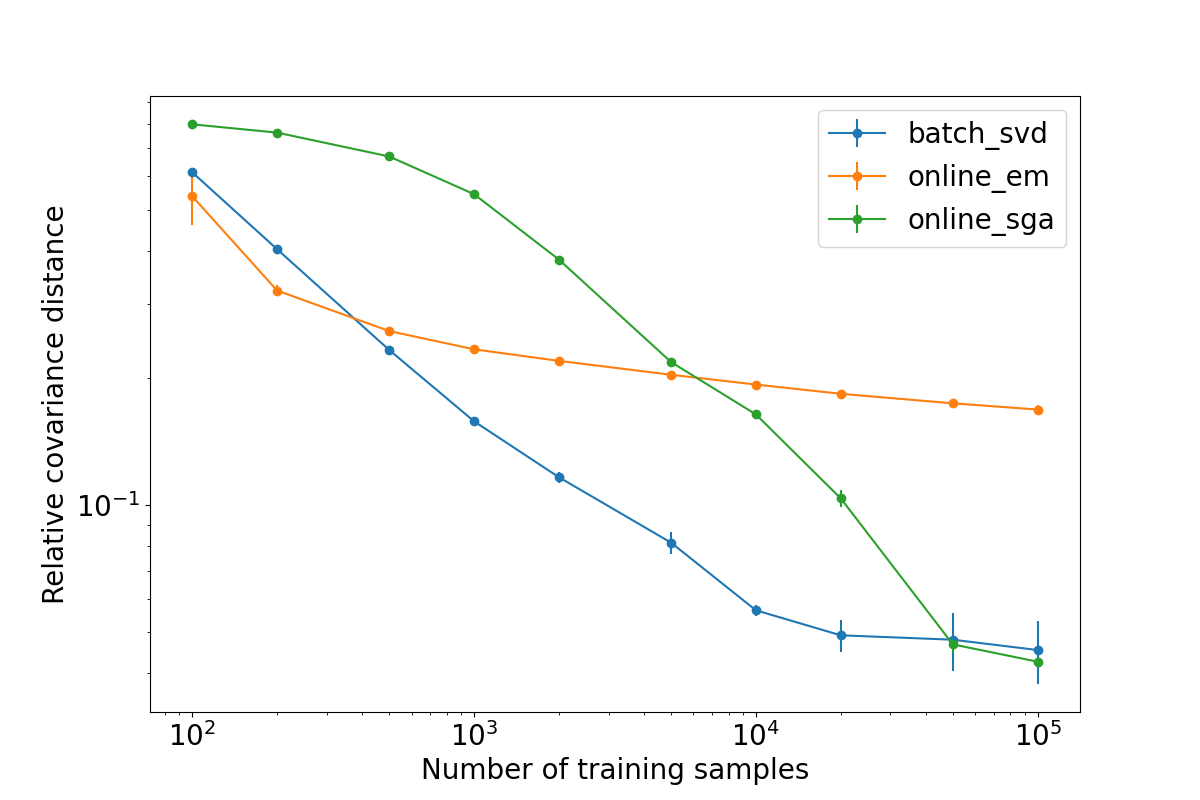
\includegraphics[width=70mm]{plots/online_fa_covar_distance__observation_dim=100__latent_dim=10__spectrum_min=1__spectrum_max=10.png}
		 & 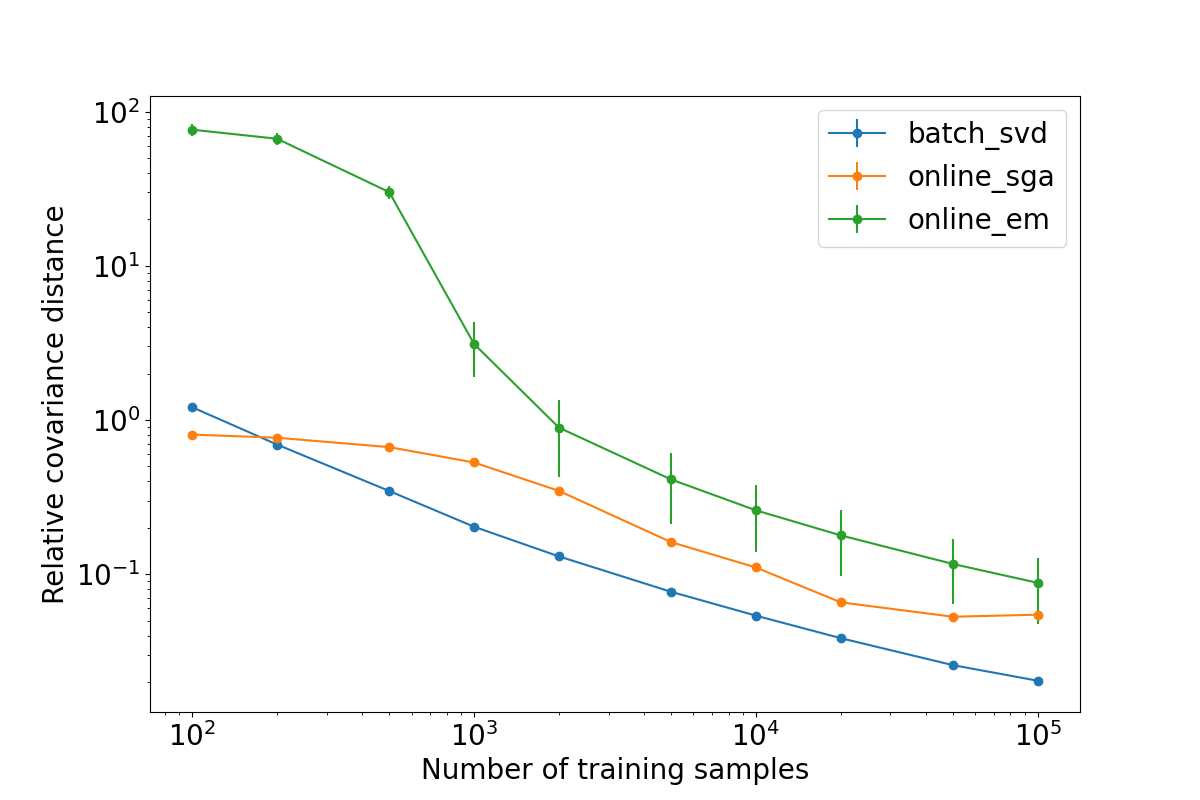
\includegraphics[width=70mm]{plots/online_fa_covar_distance__observation_dim=1000__latent_dim=10__spectrum_min=1__spectrum_max=10.png} \\
		 (a) $D=100$, $K=10$, $\matr{s}^2 \sim \mathcal{U}(1, 10)$ 
		 & (b) $D=1000$, $K=10$, $\matr{s}^2 \sim \mathcal{U}(1, 10)$\\[6pt]
		 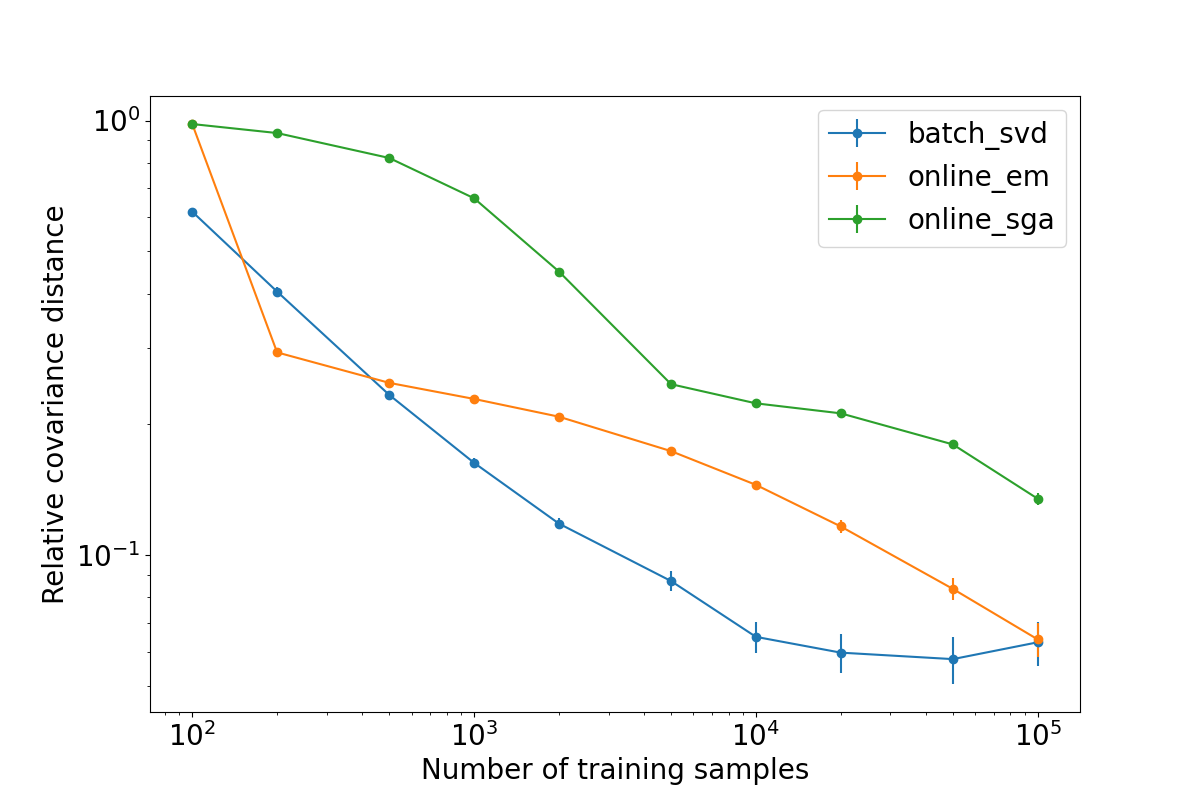
\includegraphics[width=70mm]{plots/online_fa_covar_distance__observation_dim=100__latent_dim=10__spectrum_min=1__spectrum_max=100.png}
		 & 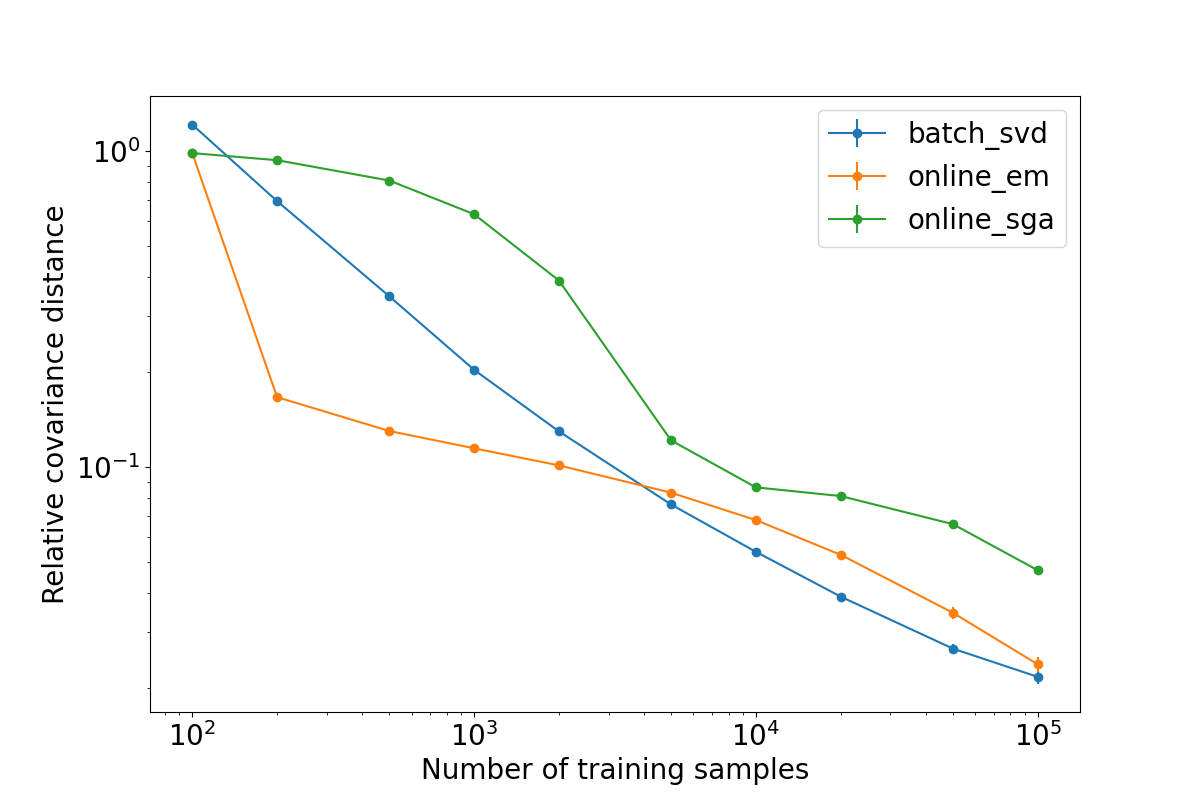
\includegraphics[width=70mm]{plots/online_fa_covar_distance__observation_dim=1000__latent_dim=10__spectrum_min=1__spectrum_max=100.png} \\
		 (c) $D=100$, $K=10$, $\matr{s}^2 \sim \mathcal{U}(1, 100)$ 
		 & (d) $D=1000$, $K=10$, $\matr{s}^2 \sim \mathcal{U}(1, 100)$\\[6pt]
		 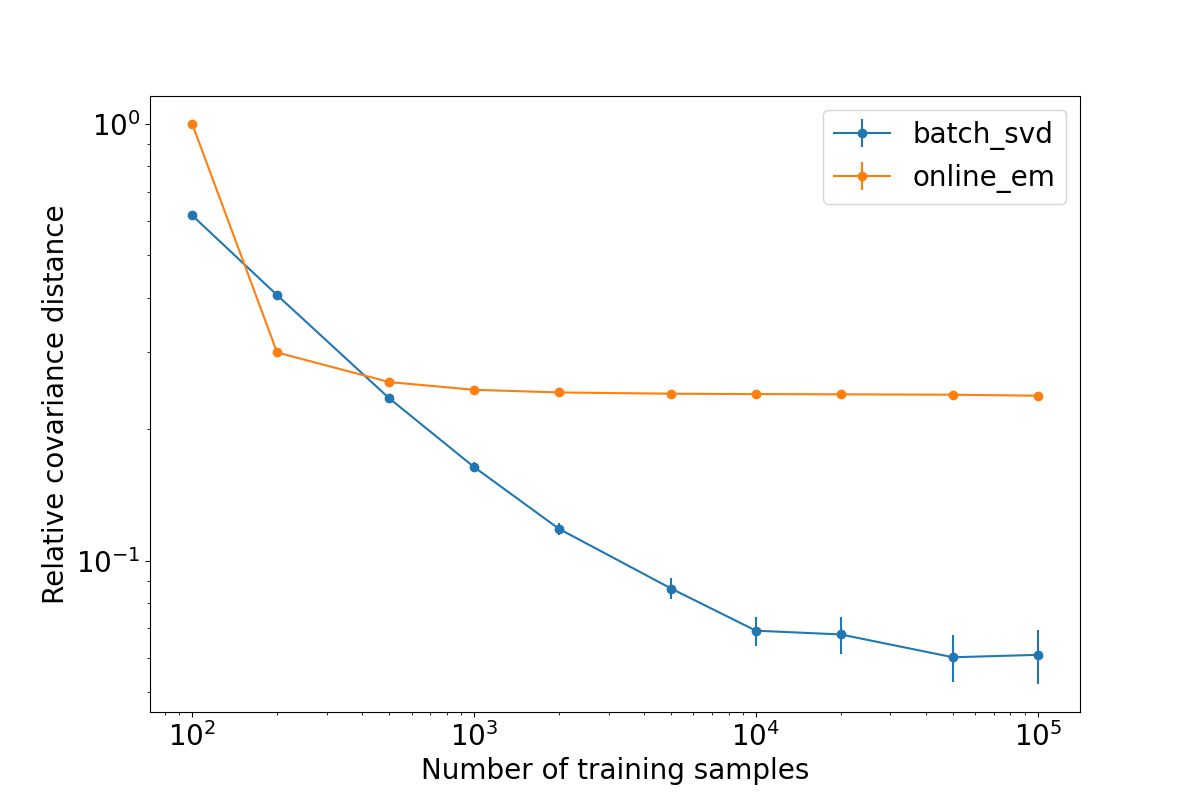
\includegraphics[width=70mm]{plots/online_fa_covar_distance__observation_dim=100__latent_dim=10__spectrum_min=1__spectrum_max=10000.png}
		 & 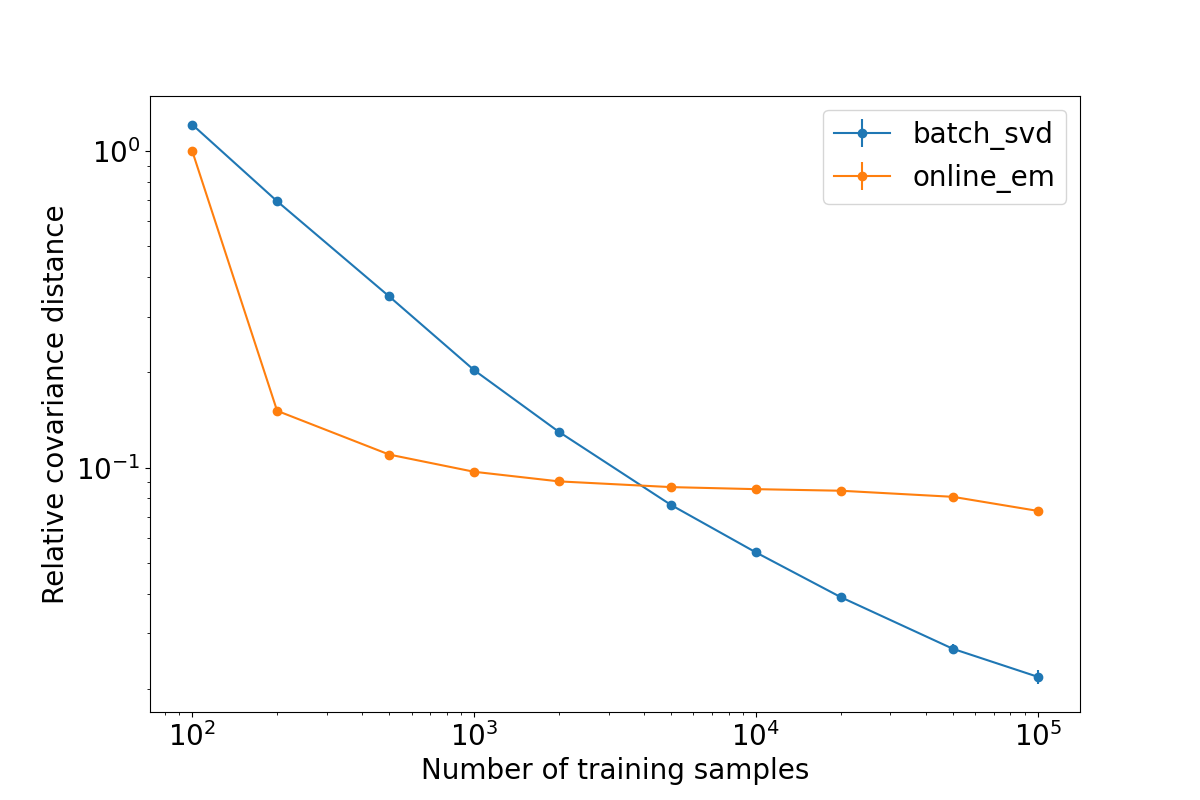
\includegraphics[width=70mm]{plots/online_fa_covar_distance__observation_dim=1000__latent_dim=10__spectrum_min=1__spectrum_max=10000.png} \\
		 (e) $D=100$, $K=10$, $\matr{s}^2 \sim \mathcal{U}(1, 10000)$ 
		 & (f) $D=1000$, $K=10$, $\matr{s}^2 \sim \mathcal{U}(1, 10000)$\\[6pt]
	\end{tabular}
	\caption{The relative distance of the estimated FA covariance matrices from the true covariance matrix as a function of the number of samples used to learn the models. The blue, orange and green lines show, for batch SVD, online EM and online SGA, respectively, the Frobenius norm of the difference between the true covariance matrix and the estimated covariance matrix divided by the Frobenius norm of the true covariance matrix. Each data point shows the mean value over ten trials with different random seeds, and standard error bars are also plotted. The different plots correspond to different combinations of the observation dimension $D$, the latent dimension $K$ and the range of the spectrum $\matr{s}^2$. The plots on the bottom row omit the results for online SGA as the distances are several orders of magnitude greater than the other results.} 
	\label{fig:fa_covar_distance}
\end{figure}


\begin{figure}[!htbp] 
	\begin{tabular}{cc}
		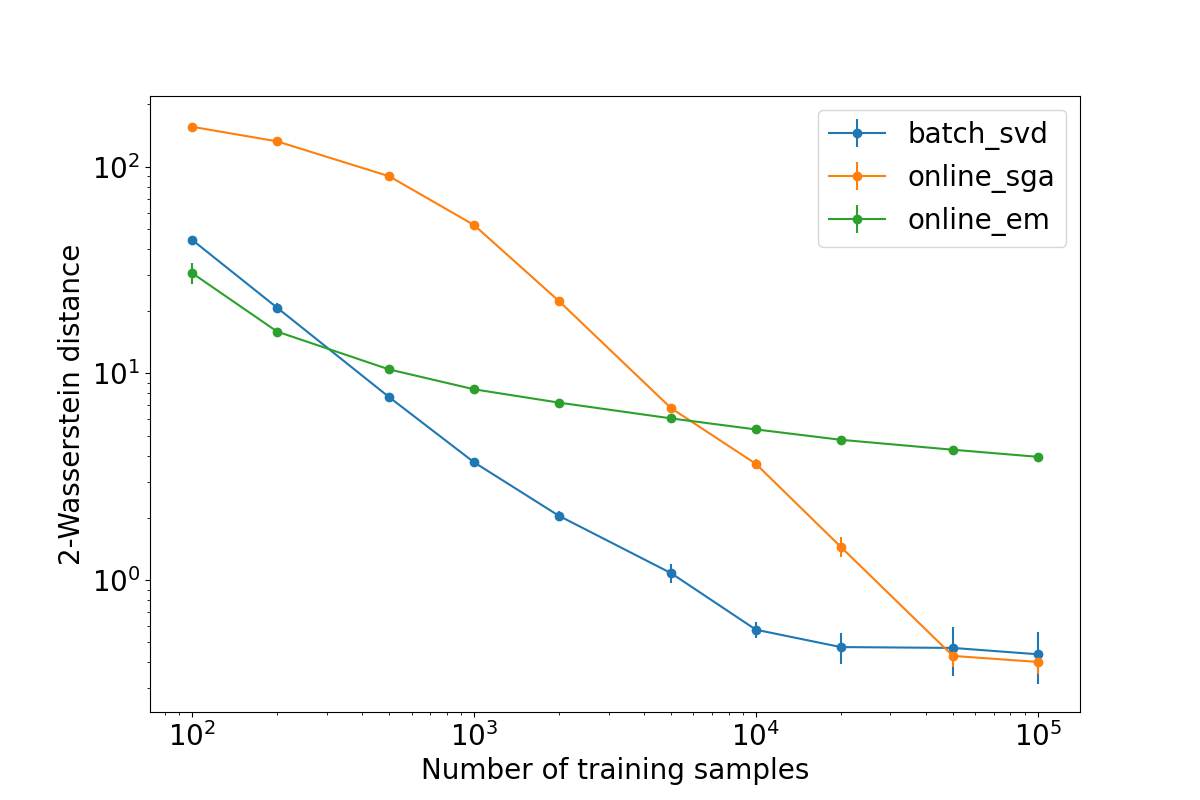
\includegraphics[width=70mm]{plots/online_fa_wasserstein__observation_dim=100__latent_dim=10__spectrum_min=1__spectrum_max=10.png}
		& 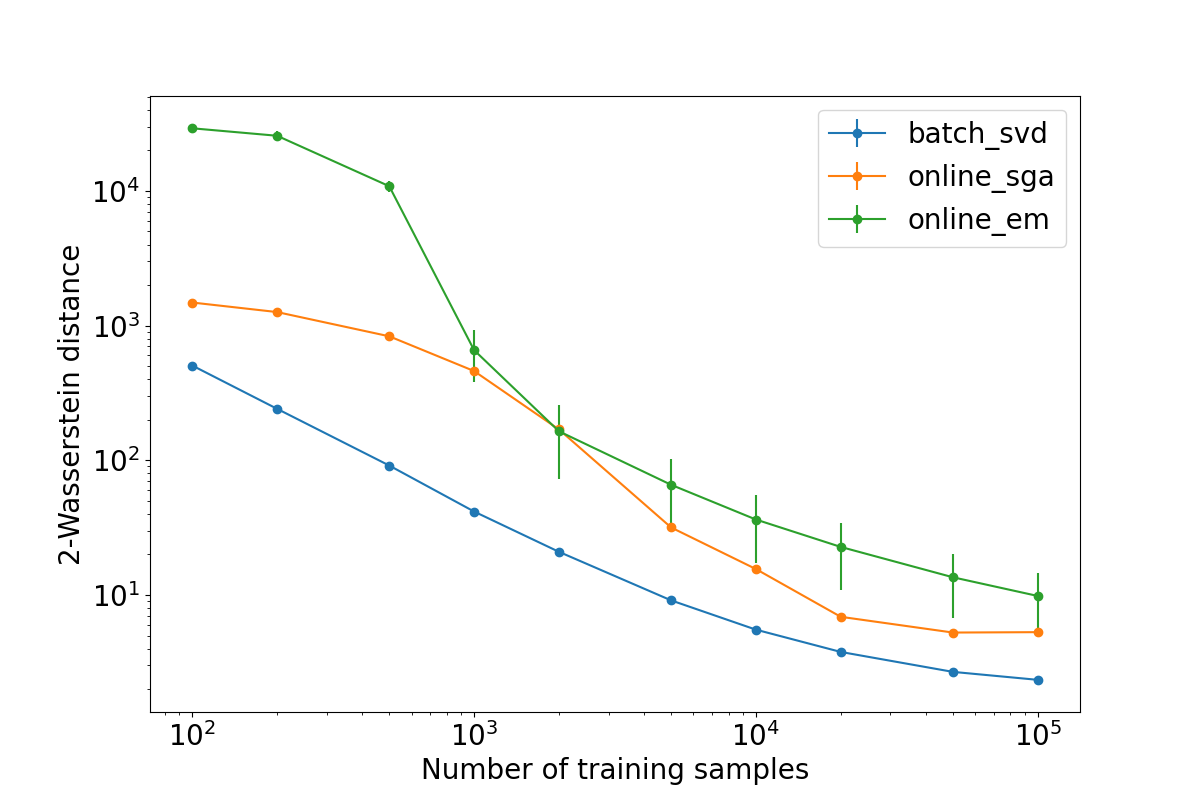
\includegraphics[width=70mm]{plots/online_fa_wasserstein__observation_dim=1000__latent_dim=10__spectrum_min=1__spectrum_max=10.png} \\
		(a) $D=100$, $K=10$, $\matr{s}^2 \sim \mathcal{U}(1, 10)$ 
		 & (b) $D=1000$, $K=10$, $\matr{s}^2 \sim \mathcal{U}(1, 10)$\\[6pt] 
		 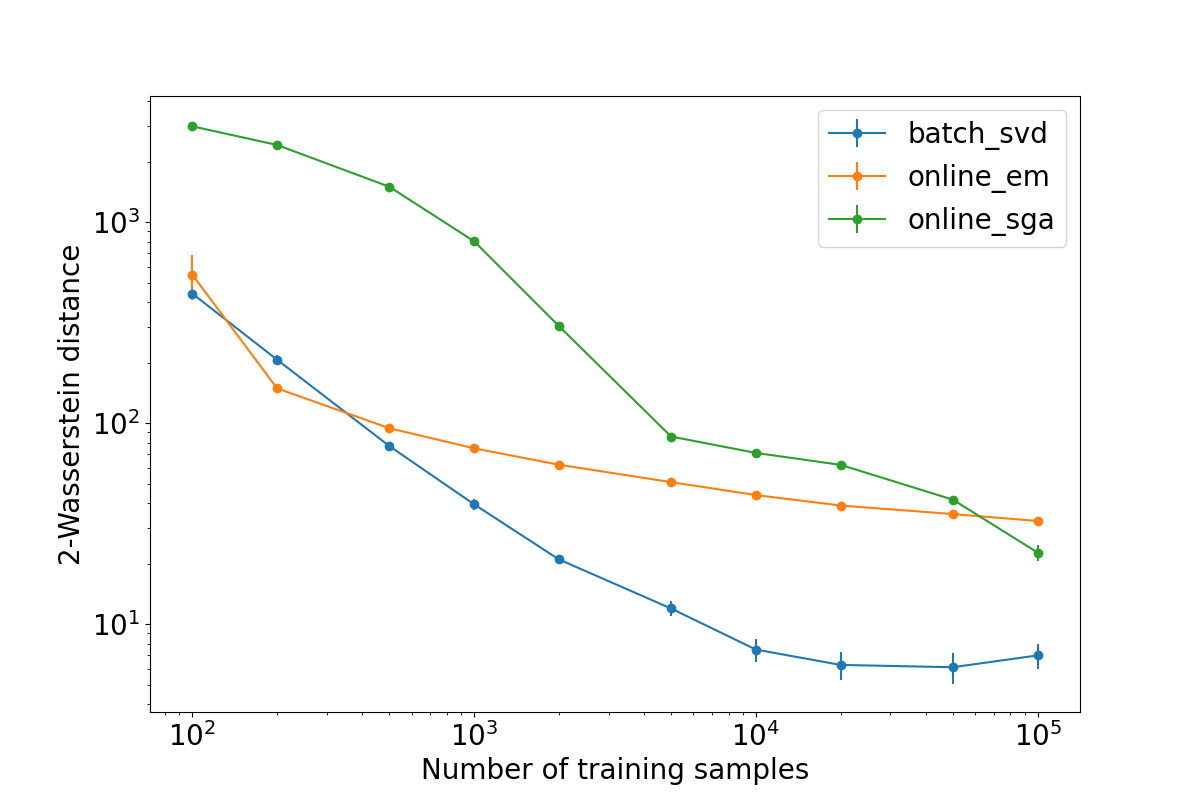
\includegraphics[width=70mm]{plots/online_fa_wasserstein__observation_dim=100__latent_dim=10__spectrum_min=1__spectrum_max=100.png} 
		 & 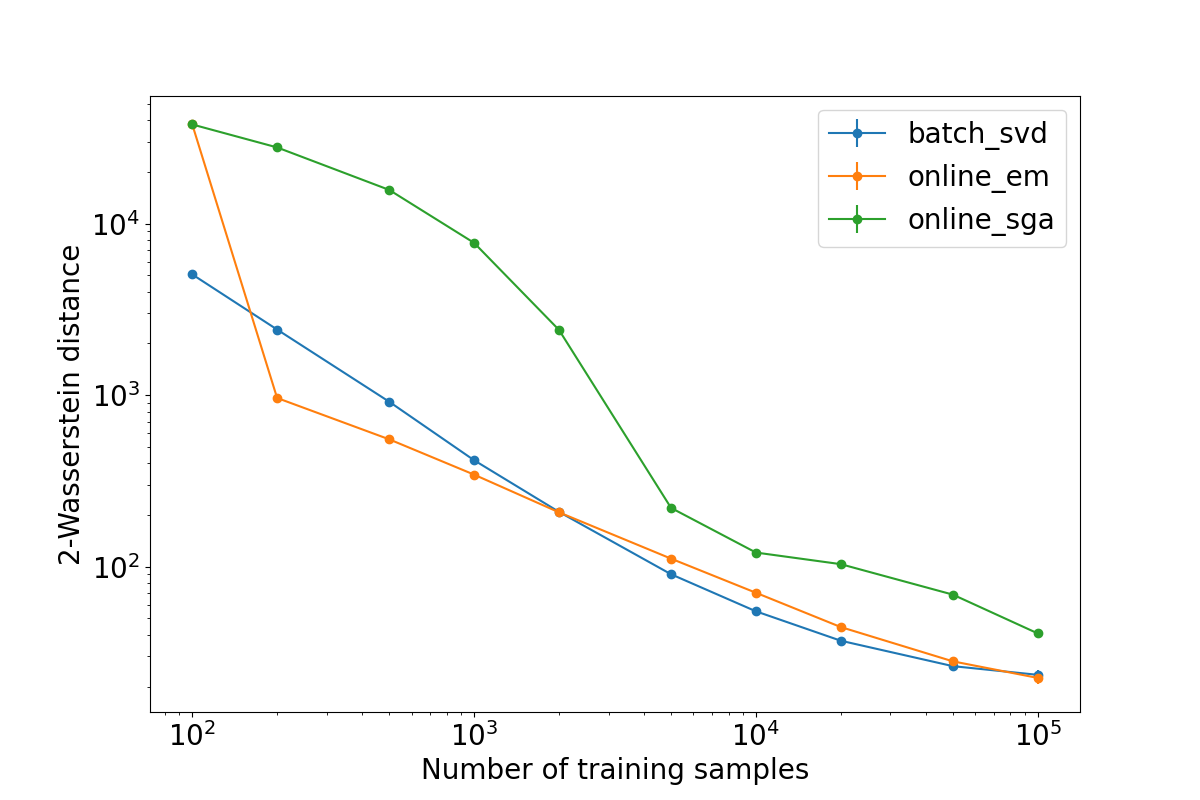
\includegraphics[width=70mm]{plots/online_fa_wasserstein__observation_dim=1000__latent_dim=10__spectrum_min=1__spectrum_max=100.png} \\
		 (c) $D=100$, $K=10$, $\matr{s}^2 \sim \mathcal{U}(1, 100)$ 
		 & (d) $D=1000$, $K=10$, $\matr{s}^2 \sim \mathcal{U}(1, 100)$\\[6pt]
		 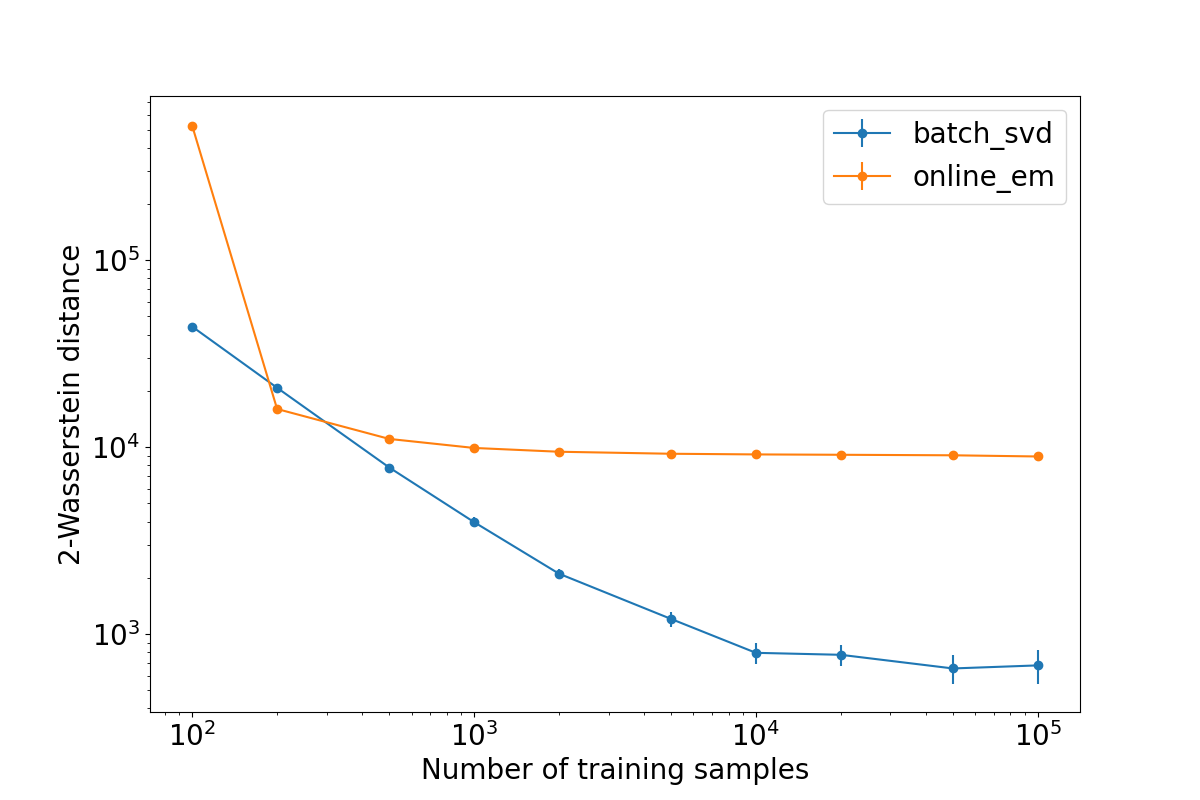
\includegraphics[width=70mm]{plots/online_fa_wasserstein__observation_dim=100__latent_dim=10__spectrum_min=1__spectrum_max=10000.png} 
		 & 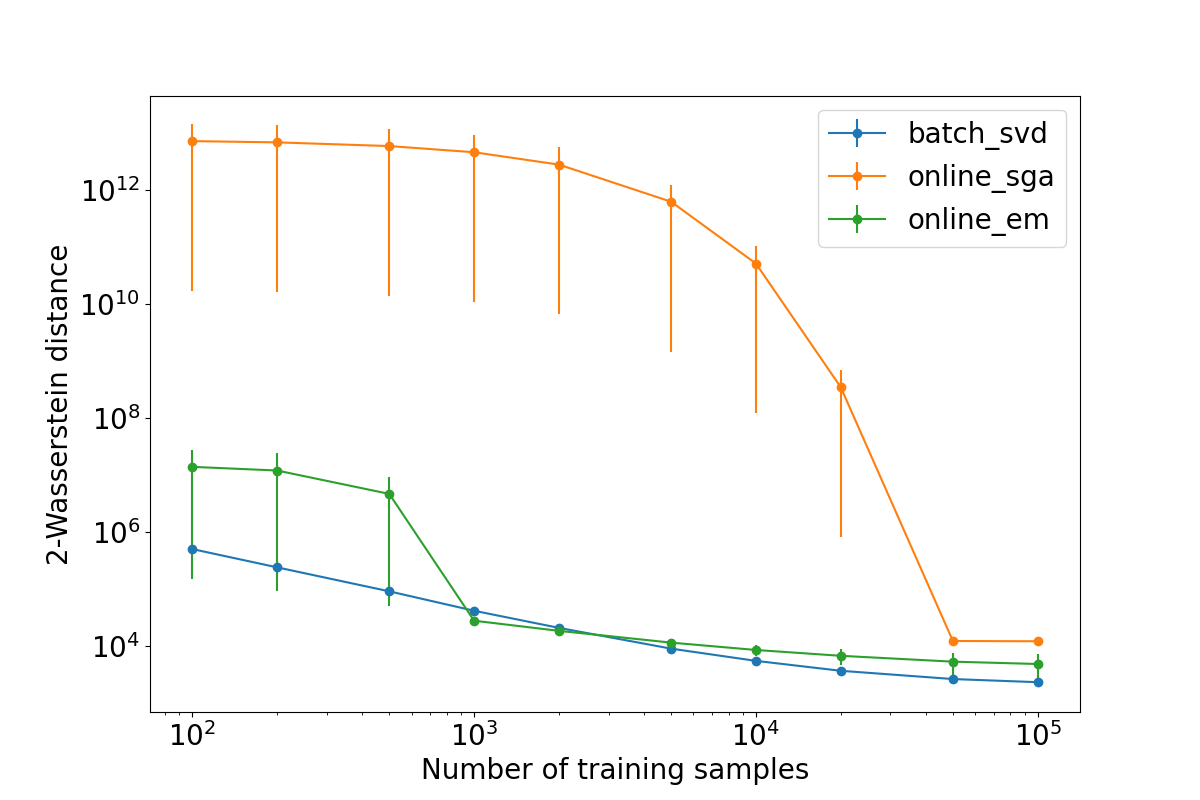
\includegraphics[width=70mm]{plots/online_fa_wasserstein__observation_dim=1000__latent_dim=10__spectrum_min=1__spectrum_max=10000.png} \\
		 (e) $D=100$, $K=10$, $\matr{s}^2 \sim \mathcal{U}(1, 10000)$ 
		 & (f) $D=1000$, $K=10$, $\matr{s}^2 \sim \mathcal{U}(1, 10000)$\\[6pt]
	\end{tabular}
	\caption{The 2-Wasserstein distance between the Gaussian distribution defined by the estimated FA model and the Gaussian distribution defined by the true FA model. The blue, orange and green lines show the 2-Wasserstein distance corresponding to batch SVD, online EM and online SGA, respectively. Each data point shows the mean value over ten trials with different random seeds, and standard error bars are also plotted. The different plots correspond to different combinations of the observation dimension $D$, the latent dimension $K$ and the range of the spectrum $\matr{s}^2$. The plots on the bottom row omit the results for online SGA as the distances are several orders of magnitude greater than the other results.}
	\label{fig:fa_wasserstein}
\end{figure}


\chapter{Linear Regression Experiments}\label{ch:linear_regression_experiments}

Since the posterior of the linear regression parameter vector can be computed in closed form, the ability of the online FA algorithms to learn the posterior can be evaluated in this case. For a linear regression model trained via SGD, Algorithms \ref{alg:gradient_fa} and \ref{alg:online_em} can both be used to fit a Gaussian posterior distribution to the iterates, $\theta_1, \dots, \theta_T$, encountered along the SGD trajectory. The mean and covariance of the learned distributions can then be compared directly to the ground truth. Recall, however, that the posterior distribution in Equation (\ref{eqn:linear_regression_posterior}) refers to specific values of $\alpha$ and $\beta$. The parameter $\beta$ is $\frac{1}{\sigma^2}$, where $\sigma$ is the standard deviation of the outputs $y_n$ in Equation (\ref{eqn:linear_regression_pdf}). This can be estimated by calculating the empirical standard deviation of $\{y_n\}_{n=1}^{N}$. 

The precision $\alpha$ is a hyperparameter which controls the width of the prior $p(\theta)$. In Equation (\ref{eqn:linear_regression_log_posterior}), the log-posterior of $\theta$ was written as 
\begin{equation}
	\log p(\theta | \mathcal{D}) 
	= -\frac{\beta}{2} \sum_{n=1}^N \big(y_n - \theta^\intercal \matr{x}_n \big)^2 
	-\frac{\alpha}{2} \theta^\intercal \theta 
	+ \text{constant}.
\end{equation}
Hence, the maximum \emph{a posteriori} (MAP) estimate of $\theta$ is that which maximises
\begin{equation}
	-\frac{\beta}{2} \sum_{n=1}^N \big(y_n - \theta^\intercal \matr{x}_n \big)^2 
	-\frac{\alpha}{2} \theta^\intercal \theta.
\end{equation}
Since $\beta > 0$, it is equivalent to minimise this expression scaled by $-\frac{2}{\beta}$, that is,
\begin{equation}
	\sum_{n=1}^N \big(y_n - \theta^\intercal \matr{x}_n \big)^2 
	+ \frac{\alpha}{\beta} \theta^\intercal \theta.
\end{equation}
This objective function is analogous to the L2-regularised training loss often used in non-Bayesian linear regression \cite{barber2007}, which is 
\begin{equation}\label{eqn:regularised_linear_regression}
	\sum_{n=1}^N \big(y_n - \theta^\intercal \matr{x}_n \big)^2 
	+ \lambda \theta^\intercal \theta 
\end{equation}
for some $\lambda > 0$. Setting $\lambda = \frac{\alpha}{\beta}$, the optimal $\theta$ found by L2-regularised linear regression is the same as the MAP estimate of $\theta$ in Bayesian linear regression with prior $p(\theta) = \mathcal{N}\big(\matr{0}, \alpha^{-1} \matr{I} \big)$. This means that, given data $\mathcal{D}$ and a particular value of $\alpha$, the posterior distribution of $\theta$ can be estimated by fitting an online FA model to the SGD iterates sampled while minimising Equation (\ref{eqn:regularised_linear_regression}) with $\lambda = \frac{\alpha}{\beta}$.
 
\section{Methodology}

The aim of these experiments is to test how well the online FA algorithms, fit to the weight vectors sampled during SGD while training a linear regression model, are able to approximate the true posterior distribution of the weights. For this purpose, four real regression datasets from the UCI Machine Learning Repository \cite{dua2019} were used. Namely, the Boston Housing\footnote{https://archive.ics.uci.edu/ml/machine-learning-databases/housing}, Concrete Compressive Strength\footnote{https://archive.ics.uci.edu/ml/datasets/concrete+compressive+strength}, Energy Efficiency\footnote{https://archive.ics.uci.edu/ml/datasets/energy+efficiency} and Yacht Hydrodynamics\footnote{http://archive.ics.uci.edu/ml/datasets/yacht+hydrodynamics} datasets. More details about these datasets are given in Table \ref{table:uci_datasets}. Note that the Energy Efficiency dataset has two target variables, heating load and cooling load, but in these experiments only the heating load was used. 

\begin{table}[h!]
	\begin{center}
		\begin{tabular}{||c c c ||} 
 			\hline
 			Dataset & No. of Instances & No. of Input Variables \\ [0.5ex] 
 			\hline\hline
 			Boston Housing & 506 & 13 \\ 
 			\hline
 			Concrete Compressive Strength & 1030 & 8 \\
 			\hline
 			Energy Efficiency & 768 & 8 \\
 			\hline
 			Yacht Hydrodynamics & 308 & 6 \\ [1ex] 
 			\hline
		\end{tabular}
		\caption{UCI regression datasets used in experiments with linear models.}
		\label{table:uci_datasets}
	\end{center}
\end{table}

In each experiment, a linear regression model was trained on one of these datasets via mini-batch SGD for 1000 epochs, with a batch size of 32. The L2 regularisation strength was set to $\lambda = \frac{\alpha}{\beta}$. Recall that $\beta$ is just the reciprocal of the variance of the target variable and $\alpha$ is a hyperparameter which controls the width of the prior on the linear regression weights. Both $\alpha$ and $\beta$ are used when computing $\matr{A}$ in Equation \ref{eqn:linear_model_A_and_b}. In order to balance the effect of the prior term and the data term, $\alpha$ was set to $0.01$ times the mean of the diagonal entries of $\beta \sum_{n=1}^N \matr{x}_n \matr{x}_n^\intercal$.

Before training began, the factors of two FA models were initialised as described in Section \ref{sec:F_init}. Their observation dimension was set to the number of weights in the linear regression model, as their purpose was to approximate the posterior distribution of the weights. After an initial warm-up period of training the linear model for 10 epochs, the two FA models began to be updated, one via online SGA and the other via online EM (Algorithms \ref{alg:gradient_fa} and \ref{alg:online_em}, respectively). An update to each FA model was performed using the weight vector sampled after each mini-batch update to the linear model. As in the experiments in Chapter \ref{ch:online_fa_experiments}, $\matr{F}$ and $\Psi$ remained fixed during the first 100 updates to the FA models, with only the running average being updated in this period. The SGA updates were performed with a learning rate of 0.001. 

The mean and covariance of the true posterior of the linear regression weights, for the specific values of $\alpha$ and $\beta$, were computed prior to training according to Equation \ref{eqn:linear_regression_posterior_params}. After each set of 10 training epochs, the distance between the parameters of the true posterior and the posteriors estimated by the online FA algorithms was computed. For each dataset, this experiment was run with the latent dimension of the FA models set to $K=1, 2, 3$. Each experiment was repeated ten times. In each trial a different random seed was used for initialising the weights of the linear model and also initialising the parameters of the FA models.

\section{Results}


%Figures \ref{fig:linear_models_empirical_boston_housing}, \ref{fig:linear_models_empirical_concrete_strength}, \ref{fig:linear_models_empirical_energy_efficiency} and \ref{fig:linear_models_empirical_yacht_hydrodynamics} show the results for the Boston Housing, Concrete Compressive Strength, Energy Efficiency and Yacht Hydrodynamics datasets, respectively. 
%
%\begin{figure}[!htbp] 
%	\centering
%	\begin{tabular}{cc}
%		\includegraphics[width=140mm]{plots/linear_models_empirical_covar_distance__boston_housing} \\
%		\includegraphics[width=140mm]{plots/linear_models_empirical_wasserstein__boston_housing} 
%	\end{tabular}
%	\caption{Learning the empirical covariance matrix of the weight vectors sampled during SGD while training a linear model on the \textbf{Boston Housing} dataset. Results for batch SVD, online SGA and online EM are show in the left, centre and right axes, respectively. \textbf{Top row}: the Frobenius norm of the difference between the empirical covariance matrix and the learned covariance matrix, divided by the Frobenius norm of the empirical covariance matrix. \textbf{Bottom row}: the 2-Wasserstein distance between the empirical Gaussian distribution and the learned Gaussian distribution. Each line corresponds to a different latent dimension for the learned FA models. Each data point shows the mean value over ten trials with different random seeds, and standard error bars are also plotted.}
%	\label{fig:linear_models_empirical_boston_housing}
%\end{figure}
%
%
%\begin{figure}[!htbp] 
%	\centering
%	\begin{tabular}{cc}
%		\includegraphics[width=140mm]{plots/linear_models_empirical_covar_distance__concrete_strength} \\
%		\includegraphics[width=140mm]{plots/linear_models_empirical_wasserstein__concrete_strength} 
%	\end{tabular}
%	\caption{Learning the empirical covariance matrix of the weight vectors sampled during SGD while training a linear model on the \textbf{Concrete Compressive Strength} dataset. Results for batch SVD, online SGA and online EM are show in the left, centre and right axes, respectively. \textbf{Top row}: the Frobenius norm of the difference between the empirical covariance matrix and the learned covariance matrix, divided by the Frobenius norm of the empirical covariance matrix. \textbf{Bottom row}: the 2-Wasserstein distance between the empirical Gaussian distribution and the learned Gaussian distribution. Each line corresponds to a different latent dimension for the learned FA models. Each data point shows the mean value over ten trials with different random seeds, and standard error bars are also plotted.}
%	\label{fig:linear_models_empirical_concrete_strength}
%\end{figure}
%
%
%\begin{figure}[!htbp] 
%	\centering
%	\begin{tabular}{cc}
%		\includegraphics[width=140mm]{plots/linear_models_empirical_covar_distance__energy_efficiency} \\
%		\includegraphics[width=140mm]{plots/linear_models_empirical_wasserstein__energy_efficiency} 
%	\end{tabular}
%	\caption{Learning the empirical covariance matrix of the weight vectors sampled during SGD while training a linear model on the \textbf{Energy Efficiency} dataset. Results for batch SVD, online SGA and online EM are show in the left, centre and right axes, respectively. \textbf{Top row}: the Frobenius norm of the difference between the empirical covariance matrix and the learned covariance matrix, divided by the Frobenius norm of the empirical covariance matrix. \textbf{Bottom row}: the 2-Wasserstein distance between the empirical Gaussian distribution and the learned Gaussian distribution. Each line corresponds to a different latent dimension for the learned FA models. Each data point shows the mean value over ten trials with different random seeds, and standard error bars are also plotted.}
%	\label{fig:linear_models_empirical_energy_efficiency}
%\end{figure}
%
%
%\begin{figure}[!htbp] 
%	\centering
%	\begin{tabular}{cc}
%		\includegraphics[width=140mm]{plots/linear_models_empirical_covar_distance__yacht_hydrodynamics} \\
%		\includegraphics[width=140mm]{plots/linear_models_empirical_wasserstein__yacht_hydrodynamics} 
%	\end{tabular}
%	\caption{Learning the empirical covariance matrix of the weight vectors sampled during SGD while training a linear model on the \textbf{Yacht Hydrodynamics} dataset. Results for batch SVD, online SGA and online EM are show in the left, centre and right axes, respectively. \textbf{Top row}: the Frobenius norm of the difference between the empirical covariance matrix and the learned covariance matrix, divided by the Frobenius norm of the empirical covariance matrix. \textbf{Bottom row}: the 2-Wasserstein distance between the empirical Gaussian distribution and the learned Gaussian distribution. Each line corresponds to a different latent dimension for the learned FA models. Each data point shows the mean value over ten trials with different random seeds, and standard error bars are also plotted.}
%	\label{fig:linear_models_empirical_yacht_hydrodynamics}
%\end{figure}


%Figures \ref{fig:linear_models_boston_housing}, \ref{fig:linear_models_concrete_strength}, \ref{fig:linear_models_energy_efficiency} and \ref{fig:linear_models_yacht_hydrodynamics} show the results for the Boston Housing, Concrete Compressive Strength, Energy Efficiency and Yacht Hydrodynamics datasets, respectively. 
%
%\begin{figure}[!htbp] 
%	\centering
%	\begin{tabular}{cc}
%		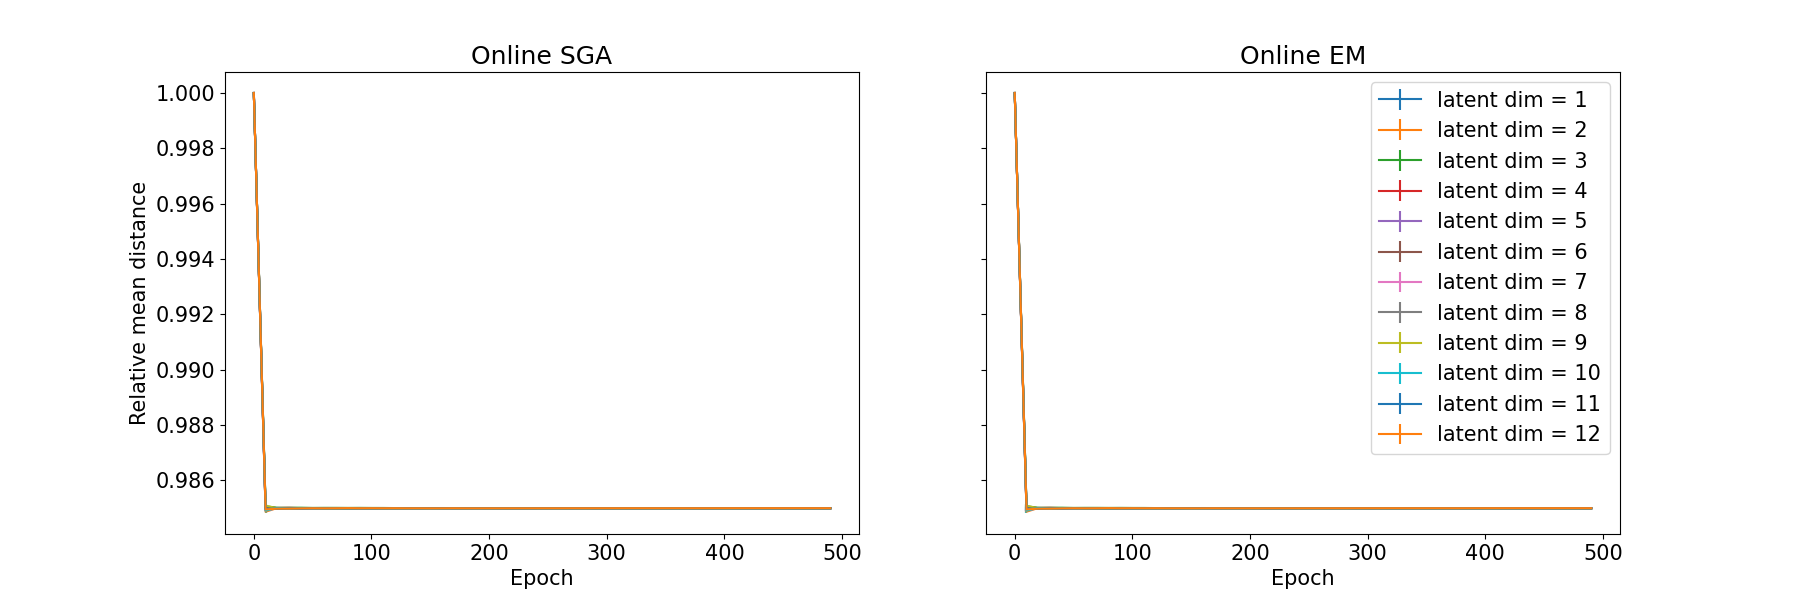
\includegraphics[width=140mm]{plots/linear_models_mean_distance__boston_housing} \\
%		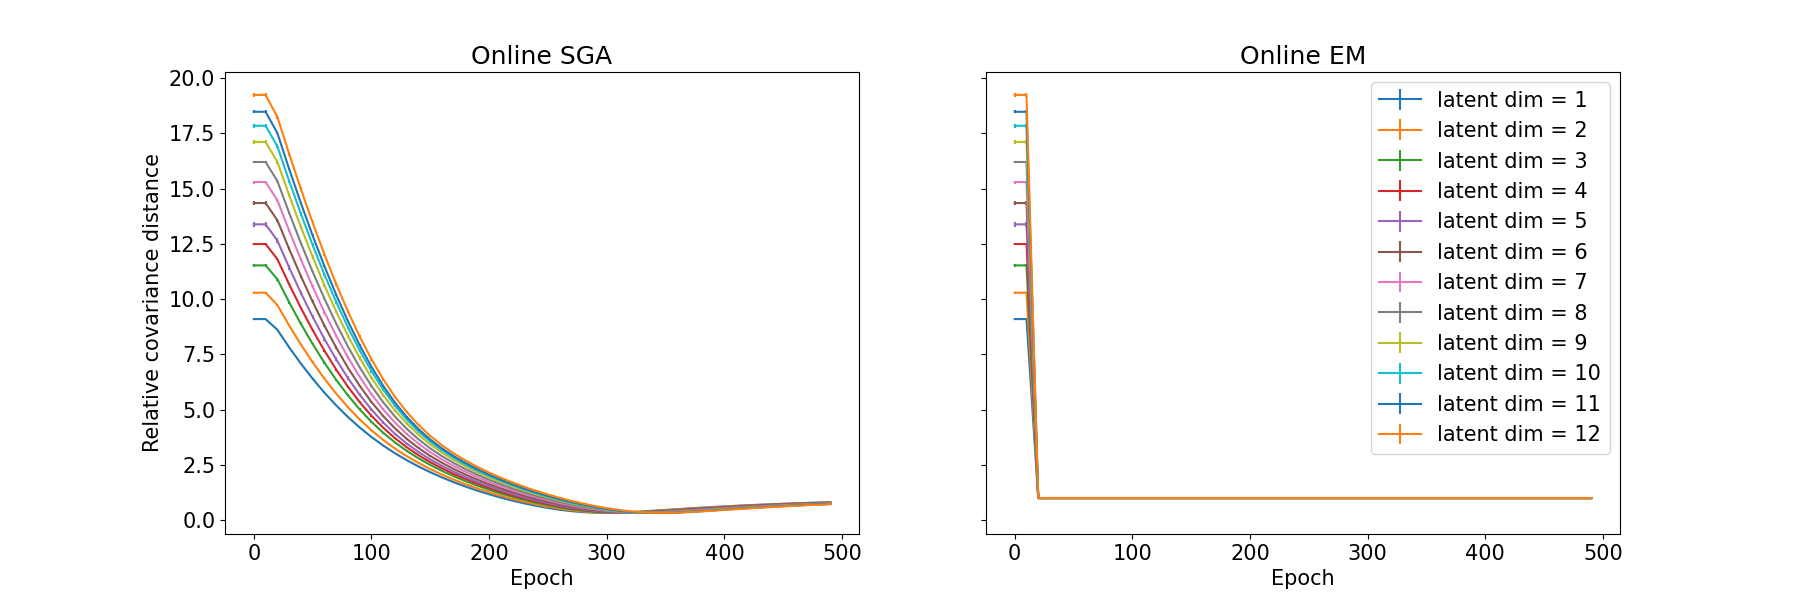
\includegraphics[width=140mm]{plots/linear_models_covariance_distance__boston_housing} \\
%		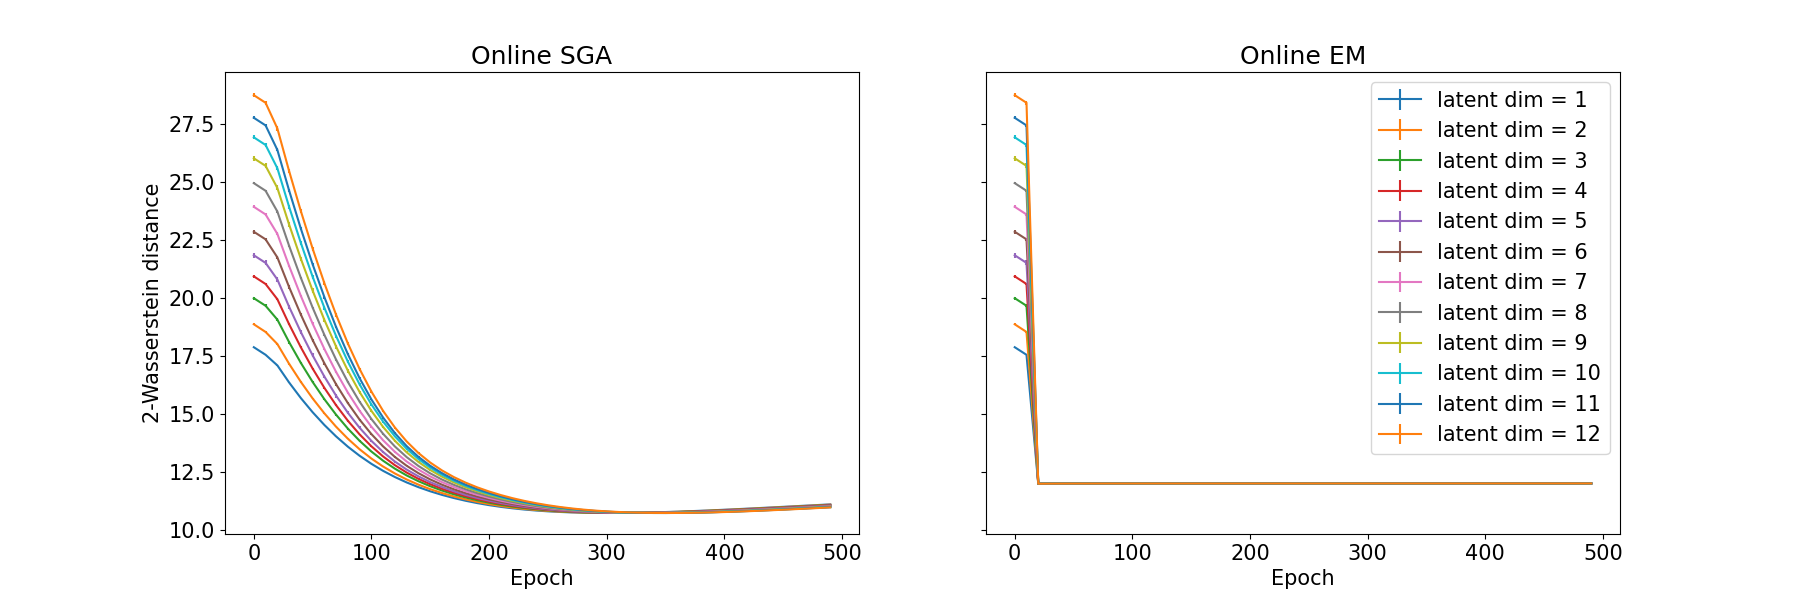
\includegraphics[width=140mm]{plots/linear_models_wasserstein__boston_housing} 
%	\end{tabular}
%	\caption{This figure show how well the online FA algorithms are able to learn the posterior distribution of the weights of a linear model trained on the \textbf{Boston Housing} dataset. Results for online SGA and online EM are show in the left and right axes, respectively. \textbf{Top row}: the Frobenius norm of the difference between the true mean and the estimated mean divided by the Frobenius norm of the true mean. \textbf{Middle row}: the Frobenius norm of the difference between the true covariance matrix and the estimated covariance matrix divided by the Frobenius norm of the true covariance matrix. \textbf{Bottom row}: the 2-Wasserstein distance between the true posterior and the estimated posterior. Each line corresponds to a different latent dimension for the learned FA models. Each data point shows the mean value over ten trials with different random seeds, and standard error bars are also plotted.}
%	\label{fig:linear_models_boston_housing}
%\end{figure}
%
%
%\begin{figure}[!htbp] 
%	\centering
%	\begin{tabular}{cc}
%		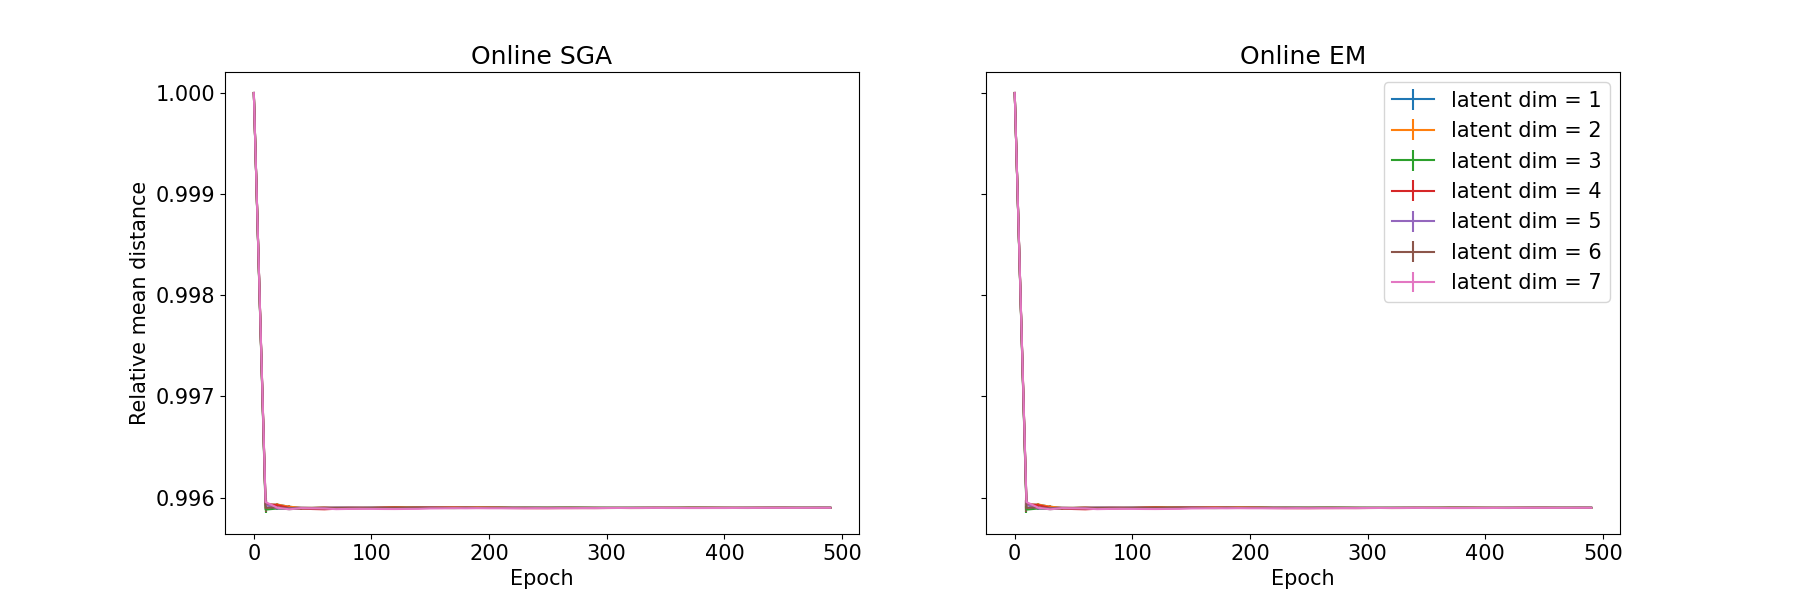
\includegraphics[width=140mm]{plots/linear_models_mean_distance__concrete_strength} \\
%		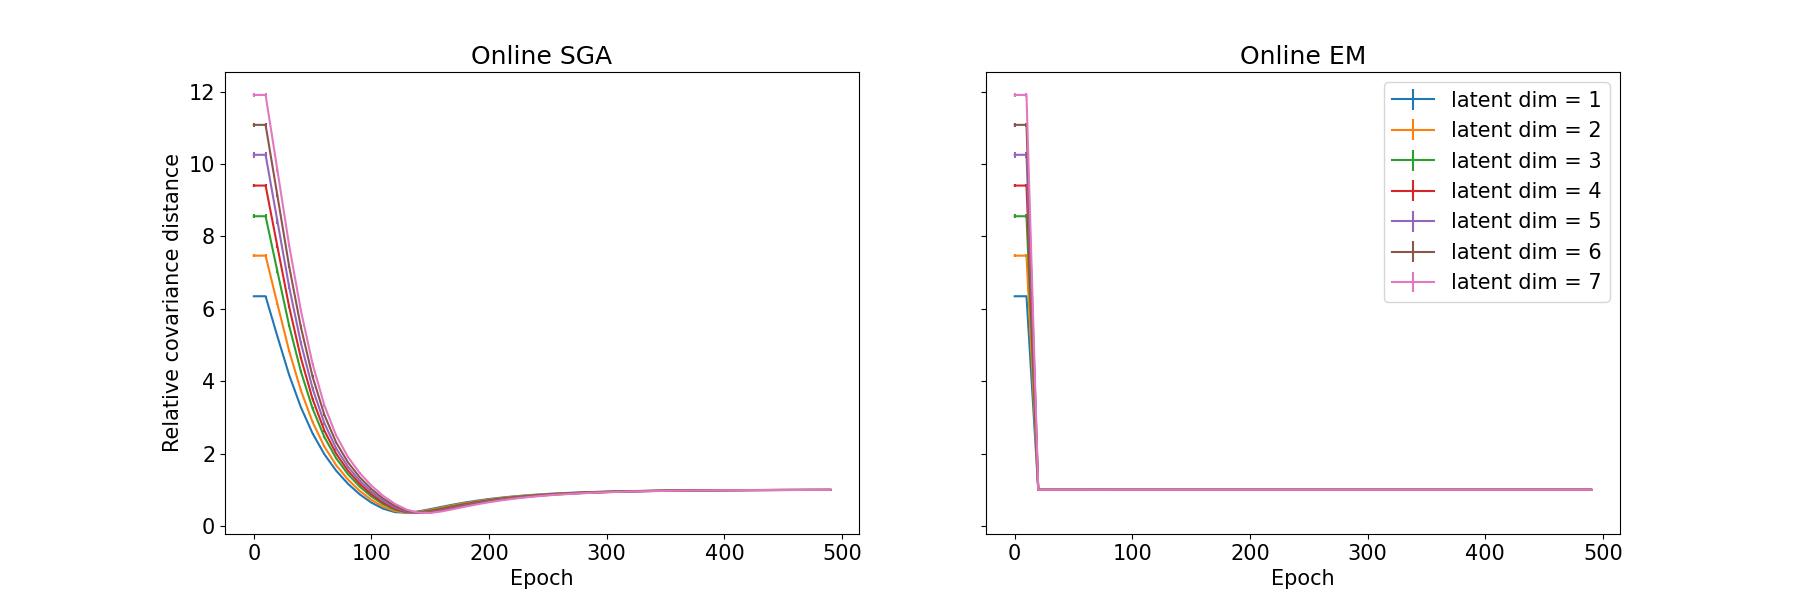
\includegraphics[width=140mm]{plots/linear_models_covariance_distance__concrete_strength} \\
%		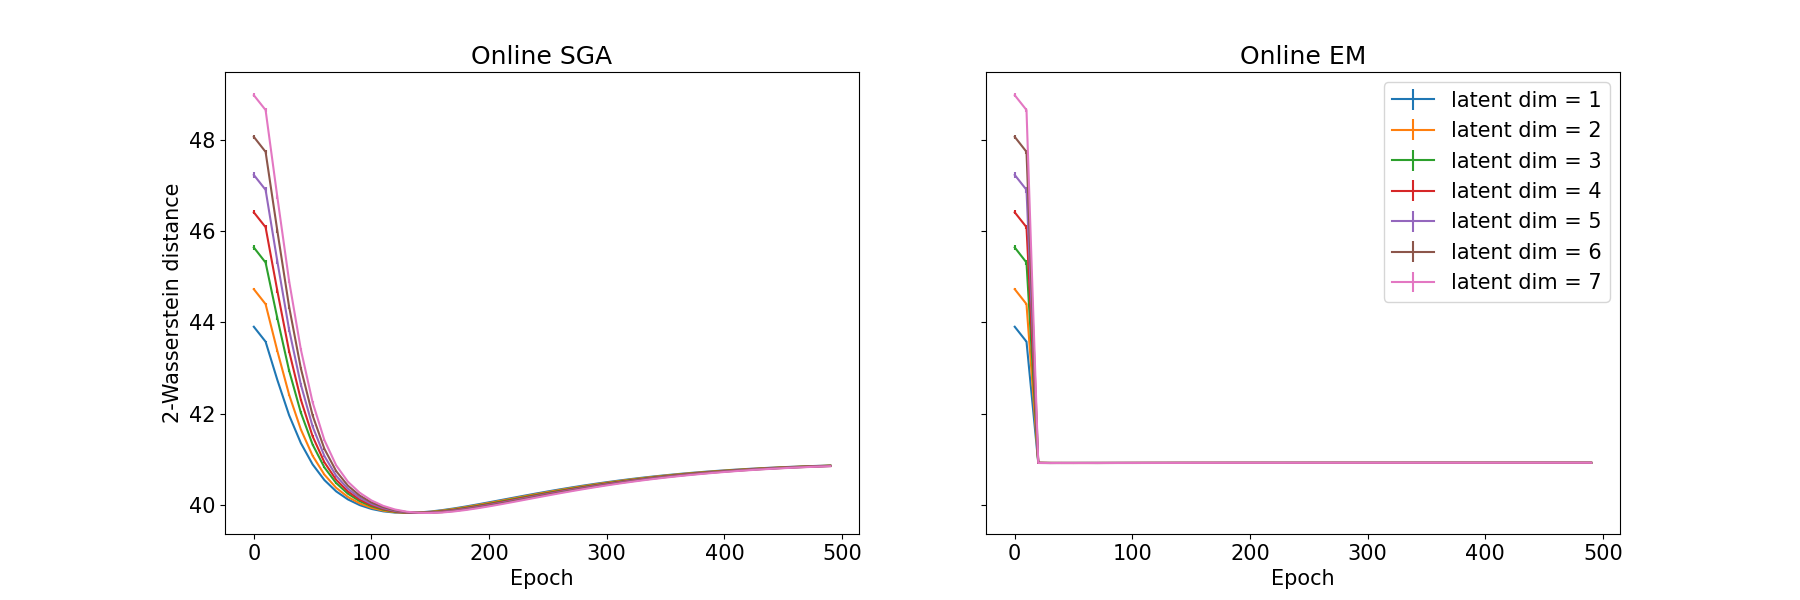
\includegraphics[width=140mm]{plots/linear_models_wasserstein__concrete_strength} 
%	\end{tabular}
%	\caption{This figure show how well the online FA algorithms are able to learn the posterior distribution of the weights of a linear model trained on the \textbf{Concrete Compressive Strength} dataset. Results for online SGA and online EM are show in the left and right axes, respectively. \textbf{Top row}: the Frobenius norm of the difference between the true mean and the estimated mean divided by the Frobenius norm of the true mean. \textbf{Middle row}: the Frobenius norm of the difference between the true covariance matrix and the estimated covariance matrix divided by the Frobenius norm of the true covariance matrix. \textbf{Bottom row}: the 2-Wasserstein distance between the true posterior and the estimated posterior. Each line corresponds to a different latent dimension for the learned FA models. Each data point shows the mean value over ten trials with different random seeds, and standard error bars are also plotted.}
%	\label{fig:linear_models_concrete_strength}
%\end{figure}
%
%
%\begin{figure}[!htbp] 
%	\centering
%	\begin{tabular}{cc}
%		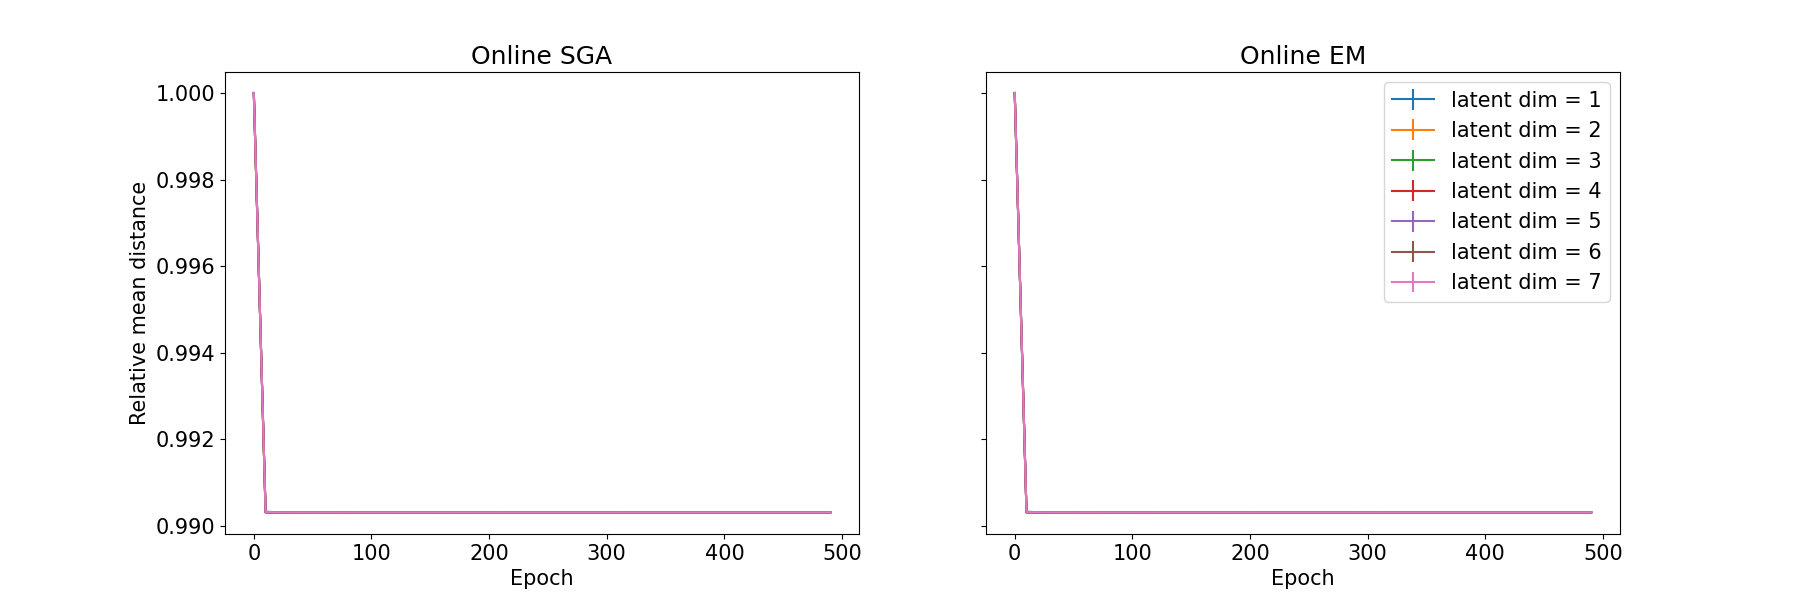
\includegraphics[width=140mm]{plots/linear_models_mean_distance__energy_efficiency} \\
%		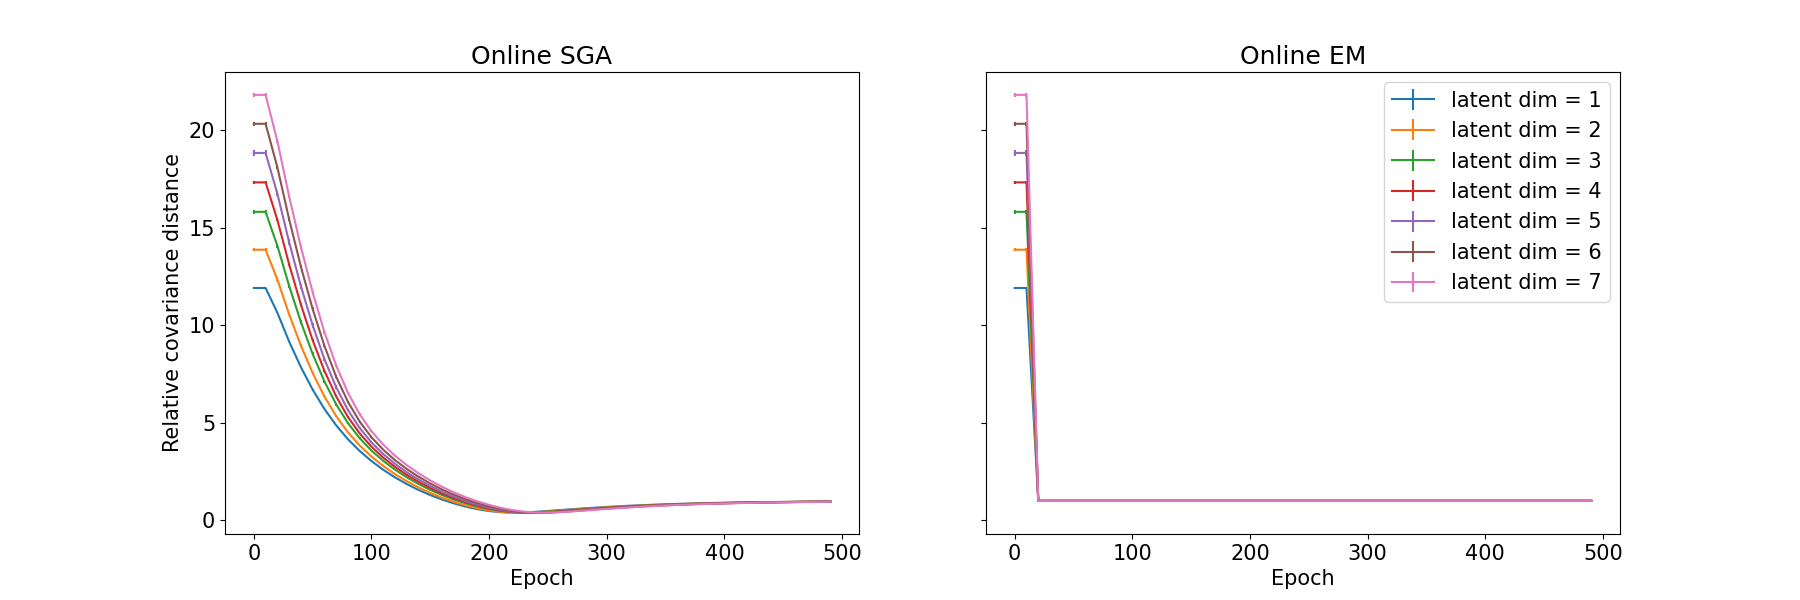
\includegraphics[width=140mm]{plots/linear_models_covariance_distance__energy_efficiency} \\
%		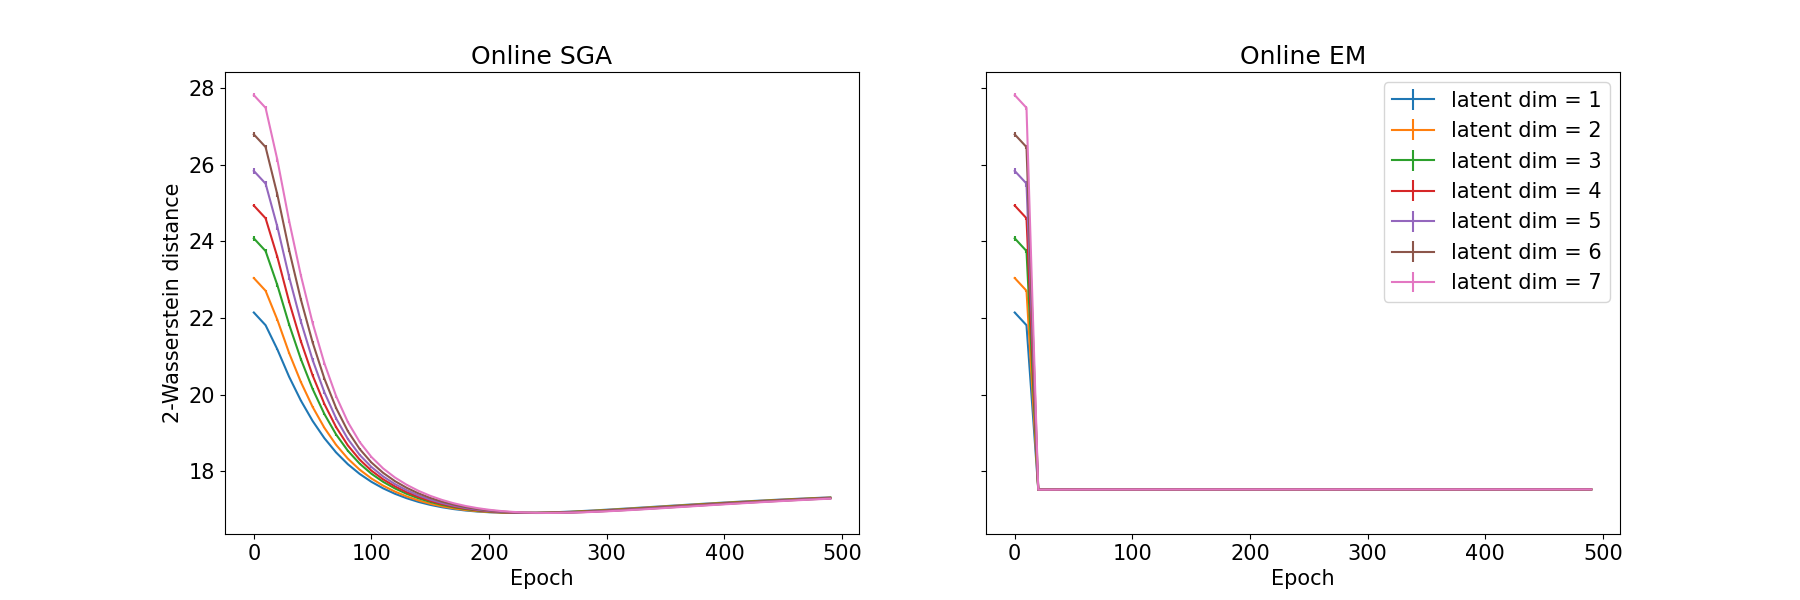
\includegraphics[width=140mm]{plots/linear_models_wasserstein__energy_efficiency} 
%	\end{tabular}
%	\caption{This figure show how well the online FA algorithms are able to learn the posterior distribution of the weights of a linear model trained on the \textbf{Energy Efficiency} dataset. Results for online SGA and online EM are show in the left and right axes, respectively. \textbf{Top row}: the Frobenius norm of the difference between the true mean and the estimated mean divided by the Frobenius norm of the true mean. \textbf{Middle row}: the Frobenius norm of the difference between the true covariance matrix and the estimated covariance matrix divided by the Frobenius norm of the true covariance matrix. \textbf{Bottom row}: the 2-Wasserstein distance between the true posterior and the estimated posterior. Each line corresponds to a different latent dimension for the learned FA models. Each data point shows the mean value over ten trials with different random seeds, and standard error bars are also plotted.}
%	\label{fig:linear_models_energy_efficiency}
%\end{figure}
%
%
%\begin{figure}[!htbp] 
%	\centering
%	\begin{tabular}{cc}
%		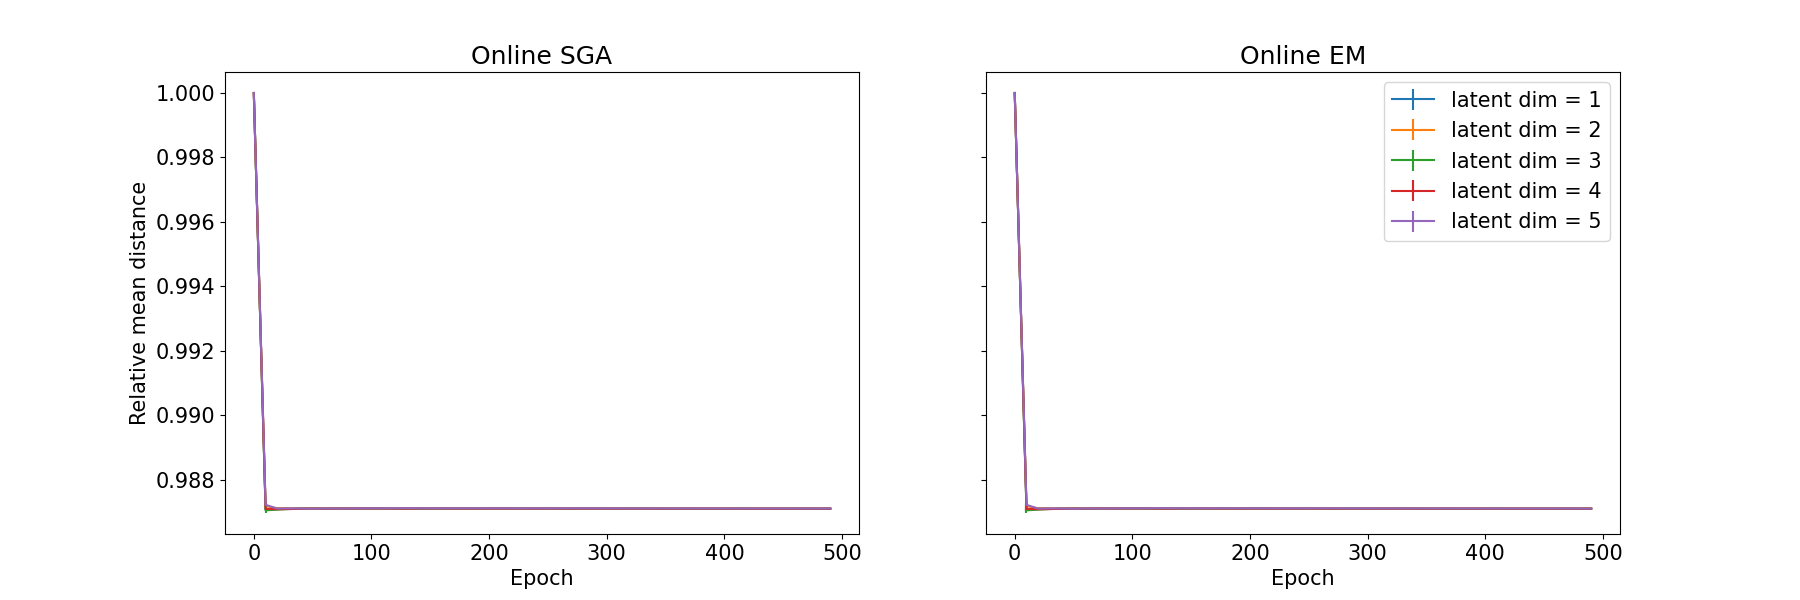
\includegraphics[width=140mm]{plots/linear_models_mean_distance__yacht_hydrodynamics} \\
%		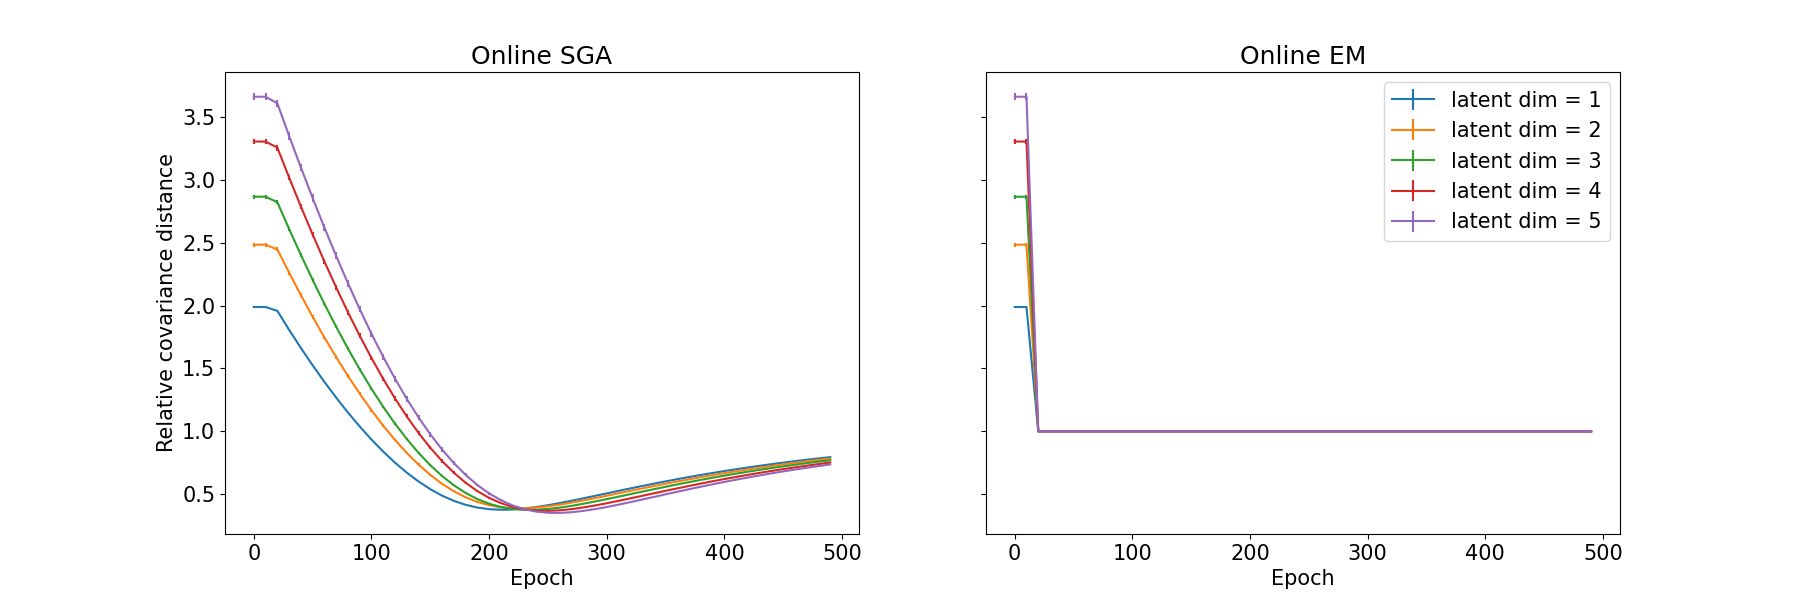
\includegraphics[width=140mm]{plots/linear_models_covariance_distance__yacht_hydrodynamics} \\
%		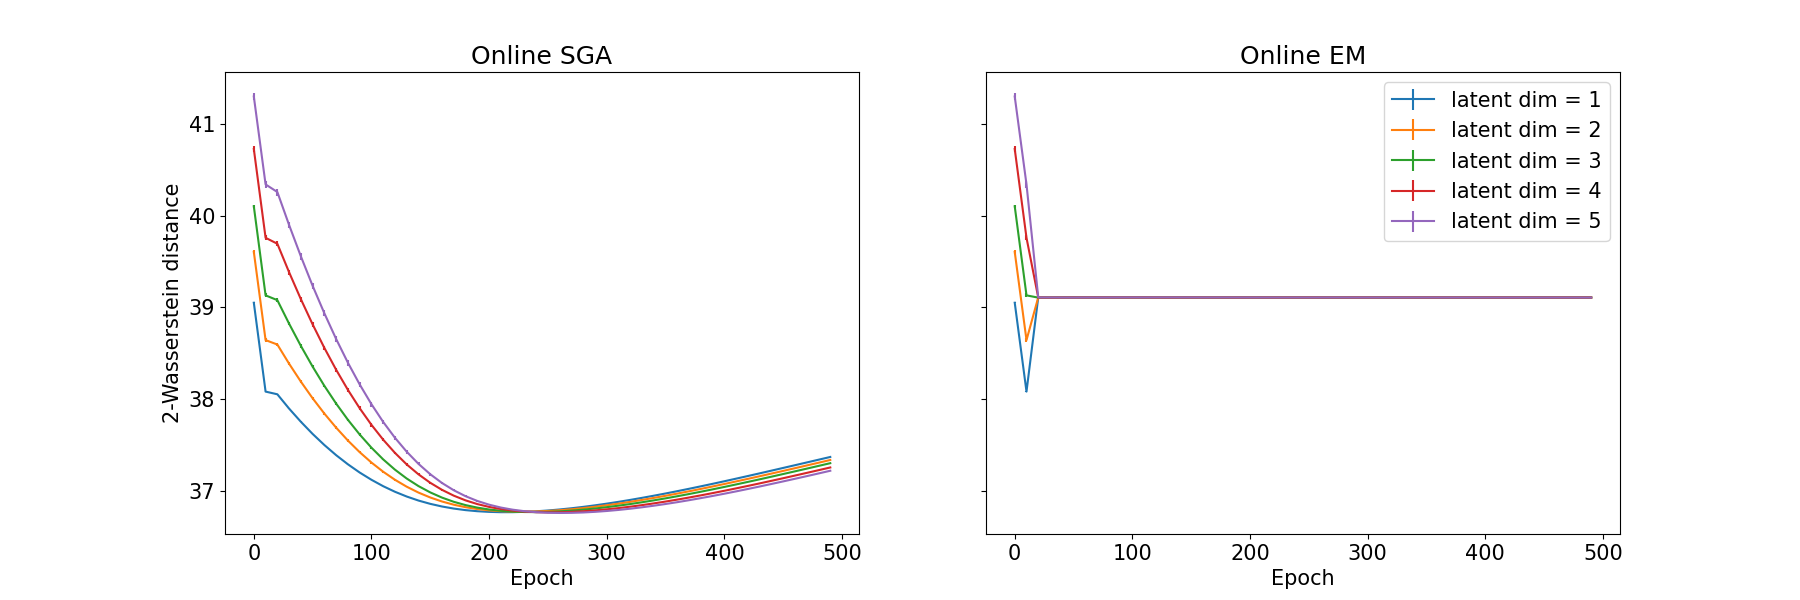
\includegraphics[width=140mm]{plots/linear_models_wasserstein__yacht_hydrodynamics} 
%	\end{tabular}
%	\caption{This figure show how well the online FA algorithms are able to learn the posterior distribution of the weights of a linear model trained on the \textbf{Yacht Hydrodynamics} dataset. Results for online SGA and online EM are show in the left and right axes, respectively. \textbf{Top row}: the Frobenius norm of the difference between the true mean and the estimated mean divided by the Frobenius norm of the true mean. \textbf{Middle row}: the Frobenius norm of the difference between the true covariance matrix and the estimated covariance matrix divided by the Frobenius norm of the true covariance matrix. \textbf{Bottom row}: the 2-Wasserstein distance between the true posterior and the estimated posterior. Each line corresponds to a different latent dimension for the learned FA models. Each data point shows the mean value over ten trials with different random seeds, and standard error bars are also plotted.}
%	\label{fig:linear_models_yacht_hydrodynamics}
%\end{figure}


\chapter{Gaussian Processes Experiments}

In was show in Section \ref{sec:gps} that, under certain conditions on the parameters, a neural network with a single, infinitely wide, hidden layer is equivalent to a GP with kernel function $k_{\text{NN}}$ given in Equation (\ref{eqn:nn_kernel}). The kernel depends on $\Sigma_{\matr{w}} \in \R^{D \times D}$, which is the covariance of the prior on the weights of each hidden unit. The individual weights of a neural network are usually independent on initialisation, so $\Sigma_{\matr{w}}$ can be set to a diagonal matrix $\sigma_w \matr{I}$. With this, $k_{\text{NN}}(\matr{x}, \matr{x}')$ can be evaluated for any two points $\matr{x}, \matr{x}' \in \R^D$. Hence, given training inputs $\matr{X} \in \R^{N\times D}$, training outputs $\matr{y} \in \R^N$ and a test point $\matr{x}_{*} \in \R^D$, the posterior predictive distribution $p(f_{*} | \matr{X}, \matr{y}, \matr{x}_{*})$ can be computed according to Equation (\ref{eqn:gp_prediction}). 

Alternatively, the Gaussian distribution $p(f_{*} | \matr{X}, \matr{y}, \matr{x}_{*})$ can be estimated via an approximate Bayesian model average (BMA). Given a posterior over the parameters of a neural network, $p(\theta |  \matr{X}, \matr{y})$, a parameter vector $\tilde{\theta} \sim p(\theta |  \matr{X}, \matr{y})$ can be used to construct a specific instance of the neural network and make a prediction for $\matr{x}_{*}$. If this procedure is repeated multiple times, the mean and variance of $p(f_{*} | \matr{X}, \matr{y}, \matr{x}_{*})$ can be estimated and compared directly to the ground truth. To obtain the parameter posterior, the online FA algorithms can be used to fit a Gaussian posterior to the iterates of the parameter vector, $\theta_1, \dots, \theta_T$, encountered while training the single layer neural network via SGD. Of course, in practice it is impossible to train a neural network with an infinitely wide hidden layer, but for these experiments it will suffice to consider neural networks with a few hundred hidden units. 


\section{Methodology}

\section{Results}

\chapter{Conclusions}

\section{Final Reminder}

The body of your dissertation, before the references and any appendices,
\emph{must} finish by page~40. The introduction, after preliminary material,
should have started on page~1.

You may not change the dissertation format (e.g., reduce the font
size, change the margins, or reduce the line spacing from the default
1.5 spacing). Over length or incorrectly-formatted dissertations will
not be accepted and you would have to modify your dissertation and
resubmit.  You cannot assume we will check your submission before the
final deadline and if it requires resubmission after the deadline to
conform to the page and style requirements you will be subject to the
usual late penalties based on your final submission time.

\bibliographystyle{plain}
\bibliography{main}

%% You can include appendices like this:
% \appendix
%
% \chapter{First appendix}
%
% \section{First section}
%
% Markers do not have to consider appendices. Make sure that your contributions
% are made clear in the main body of the dissertation (within the page limit).

\end{document}